\documentclass[11pt]{article}
\usepackage[utf8]{inputenc}
\usepackage{graphicx}
\usepackage{amssymb,amsmath,amsthm,amsfonts}
\usepackage{amsfonts}
\usepackage[usenames,dvipsnames]{color}
% \usepackage{kpfonts}
\usepackage{algorithm}
\usepackage[noend]{algorithmic}
\usepackage[square, comma, numbers,sort&compress]{natbib}
\usepackage{cleveref}
\usepackage{blindtext}
\usepackage{comment}
\newcommand{\INDSTATE}[1][1]{\STATE\hspace{#1\algorithmicindent}}
\usepackage{url}
\usepackage{comment}
\usepackage{fullpage}
\usepackage{wasysym}
\usepackage{float}
\usepackage{microtype}
\usepackage[caption=false]{subfig}
\newtheorem{claim}{Claim}
\newtheorem{fact}{Fact}
\newtheorem{observation}{Observation}
\newtheorem{lemma}{Lemma}
\newtheorem{theorem}{Theorem}

\newtheorem*{claim-non}{Claim}
\newtheorem*{theorem-non}{Theorem}


\newtheorem{corollary}{Corollary}
\newtheorem{obs}{Observation}


\makeatletter
\def\thanks#1{\protected@xdef\@thanks{\@thanks
        \protect\footnotetext{#1}}}
\makeatother


\newcommand{\app}[1]{Appendix~\ref{#1}}
\newcommand{\mute}[1]{}
%\newcommand{\mathmath}{$$ }
\newcommand{\cX}{\mathcal{X}\xspace}
\newcommand{\cA}{\mathcal{A}\xspace}
\newcommand{\cB}{\mathcal{B}\xspace}
\newcommand{\OPT}{\mathrm{OPT}}

\newcommand{\xnohatb}{\langle x, \beta \rangle}
\newcommand{\xb}{\langle \hat{x}, \beta \rangle}
\newcommand{\xbb}{\langle \hat{x}(\beta), \beta \rangle}
\newcommand{\bgb}{\beta^T G^{-1} \beta}
\newcommand{\Rd}{\mathbb{R}^d}

\newcommand{\R}{\ensuremath{\mathbb{R}}\xspace}
\newcommand{\C}{\ensuremath{\mathbb{C}}\xspace}
\newcommand{\A}{\ensuremath{\cA}\xspace}
% \renewcommand{\D}{\mathcal{D}}
\newcommand{\B}{\ensuremath{\cB}\xspace}
\newcommand{\regret}[1]{\textrm{Regret}(#1)}
\newcommand{\reg}[1]{R(#1)}
\newcommand{\pp}[2]{\pi^{#1}_{#2}}
\newcommand{\ppc}[3]{\pp{#1}{#2|#3}}
\newcommand{\rew}[2]{r^{#1}_{#2}}
\newcommand{\Rew}[2]{\D^{#1}_{#2}}
\newcommand{\bt}{\ensuremath{\bot}\xspace}
% commands for the UCB alg
\newcommand{\ist}{\ensuremath{i_{*}^t}}
\newcommand{\uit}{\ensuremath{u_{i}^t}}
\newcommand{\lit}{\ensuremath{\ell_{i}^t}}
\renewcommand{\mit}{\ensuremath{\mu_{i}^t}}
\newcommand{\mean}[2]{\ensuremath{\hat{\mu}_{#2}^{#1}}}
\newcommand{\up}[2]{\ensuremath{u_{#2}^{#1}}}
\newcommand{\low}[2]{\ensuremath{\ell_{#2}^{#1}}}
\newcommand{\num}[2]{\ensuremath{n_{#2}^{#1}}}
\newcommand{\interval}[2]{\ensuremath{[\ell_{#2}^{#1}, u_{#2}^{#1}]}}
\newcommand{\unfair}{\textrm{unfair}}
\newcommand{\fairbandits}{\textsc{FairBandits}\xspace}
\newcommand{\kwikfair}{\textsc{KWIKToFair}\xspace}
\newcommand{\fairkwik}{\textsc{FairToKWIK}\xspace}
\newcommand{\innprod}[2]{\langle{#1},{#2}\rangle}

\theoremstyle{definition}
\newtheorem{definition}{Definition}
\theoremstyle{remark}
\newtheorem{remark}{Remark}




\DeclareMathOperator*{\argmax}{arg\,max}
\DeclareMathOperator*{\argmin}{arg\,min}
\newcommand{\E}[1]{\mathbb{E}\left[ #1 \right]}
\newcommand{\Ex}[2]{\mathbb{E}_{#1}\left[ #2 \right]}
\newcommand{\I}[1]{\mathbb{I}\left[ #1 \right]}
\newcommand{\pr}[1]{\mathbb{P}\left[ #1 \right]}
\renewcommand{\Pr}[2]{\mathbb{P}_{#1}\left[ #2 \right]}



\newif \ifdraft \draftfalse
\newcommand{\zs}[1]{\ifdraft \textcolor{RedViolet}{[Zach: #1]} \fi} 
\newcommand{\abn}[1]{\ifdraft \textcolor{Green}{[Assaf: #1]} \fi}
\newcommand{\lsn}[1]{\ifdraft \textcolor{Blue}{[Lorenzo: #1]} \fi}


\title{Order-Reversal of Compactness Scores under Map Projections [DRAFT]}
\author{Assaf Bar-Natan \and Lorenzo Najt \and Zachary Schutzman }%\thanks{The authors would like to recognize the generous support of the Amar G.\ Bose Grant and the NSF GEAR Network.  Thanks to Lee Hachadoorian for inspring the original research problem and for the use of his code, and to Jeanne Clelland, Lee, Moon Duchin, Daryl DeFord, and Caleb Stanford for helpful conversations throughout the research process.}}
\begin{document}
\maketitle
	
\begin{abstract}
In political redistricting, the \textit{compactness} of a district is
used as a quantitative proxy for its fairness.  Several
well-established, yet competing, notions of geographic compactness are
commonly used to evaluate the shapes of regions, including the
\textit{Polsby-Popper score}, the \textit{convex hull score}, and the \textit{Reock score}, and
these scores are used to compare two or more districts or plans.  In
this paper, we prove mathematically that  any \textit{map
projection} from the sphere to the plane, reverses the ordering of the scores of some pair of regions for all three of these scores and many other conceivable measures as well.

\end{abstract}
\section{Introduction}\label{sec:intro}

Striving for the \textit{geometric compactness} of legislative
districts is a traditional principle of redistricting, and, to that
end, many jurisdictions have included the criterion of compactness in
their legal code for drawing districts.  However, there is no
agreed-upon definition for what makes a district compact or not.
Several competing mathematical definitions have emerged over the past
two centuries, including the \textit{Polsby-Popper score}, \cut{which
measures the ratio of a district's area to the square of its
perimeter,}  the \textit{convex hull score}, \cut{which measures the ratio
of the area of a district to the smallest convex region containing it},
and the \textit{Reock score}, \cut{which measures the ratio of the area of
a district to the smallest circle containing it}.  Each of these
measures is appealing at an intuitive level, since they each assign to
a district a single scalar value between zero and one, allowing easy
comparisons between proposed redistricting plans. Additionally, the
mathematics underpinning each is widely understandable by the relevant
parties, including lawmakers, judges, advocacy groups, and the general
public.  None of these measures is perfect, however\cit.  \cut{
For each, it is not difficult to construct a 
mathematical counterexample for which
a human's intuition and the score's evaluation of a shape's
compactness differ, such as a circle with slightly perturbed boundary
for the Polsby-Popper measure and a very long, thin rectangle for the
convex hull measure. } Additionally, these scores often do not agree.
The long, thin rectangle has a very good convex hull score, but a very
poor Polsby-Popper score.  These issues are well-studied by political
scientists and mathematicians alike
\cite{polsby1991third,frolov1975shape,maceachren1985compact}.

In this paper, we propose a further critique of these measures, namely
\textit{sensitivity under the choice of map projection}.  Each of the
compactness scores named above is defined as a tool to evaluate
geometric shapes in the plane, but in reality we are interested in
analyzing shapes which sit on the surface of the planet Earth, which
is (roughly) spherical\cit.  When a shape is assigned a compactness score,
it is implicitly done with respect to some choice of map projection.
We show, both mathematically and empirically, that this may have
serious consequences for the evaluation of compactness.  In
particular, we define the analogue of the Polsby-Popper, convex hull,
and Reock scores on the sphere, and demonstrate that for any choice of
map projection, there are two regions, $A$ and $B$, such that $A$ is
more compact than $B$ on the sphere but $B$ is more compact than $A$
when projected to the plane.

\section{Preliminaries, Spherical Geometry, Definitions, and Notation}\label{sec:prelims}

We begin by introducing some necessary observations, definitions, and terminology
which will be of use later.  
 We use $\R^2$ to denote the 
Euclidean plane with its usual metric;
similarly, $\R^3$ denotes Euclidean 3-space.  We use $\mbb{S}^2$ to denote the \textit{unit 2-sphere}, which can be 
thought of as the set of points in $\R^3$ at Euclidean distance one from the origin.  

\zs{i think saying something like this is important but the way i've written it here it's not really saying anything....}
This surface also has a `usual metric', but it is tricky to write down as a formula.   Intuitively, the distance between two points on the sphere can be found by drawing the \textit{great circle} which passes through these points and then using a circular arc length formula to compute the length of the shorter of the two segments which join the points.  
In this paper, we only consider the sphere and the plane, and leave the consideration of other surfaces, measures, and metrics to future work.










\begin{definition}
	In a metric space, a \textbf{geodesic} between two points is the shortest path connecting them with respect to the metric.
	In the plane, geodesics are line segments, and on the surface of the sphere, geodesics are segments of great circles.
\end{definition}





Geodesics are intricately tied to the metric of the space we're working with, because one way to think of the metric distance between two points is as the length of the shortest geodesic connecting them.  We also note that in the plane, there is a \textit{unique} line segment between any two distinct points, whereas on the sphere, there are two such geodesic segments.  This leads to the definition of a \textit{spherical line}.


\begin{definition}
	On the sphere, the lines are \textit{great circles}, which are the circles of the largest possible radius on the surface of the sphere.  Equivalently, they are the intersections of the surface of the sphere with a plane passing through the center of the sphere.
\end{definition}  

\begin{figure}[htb]
	\centering
	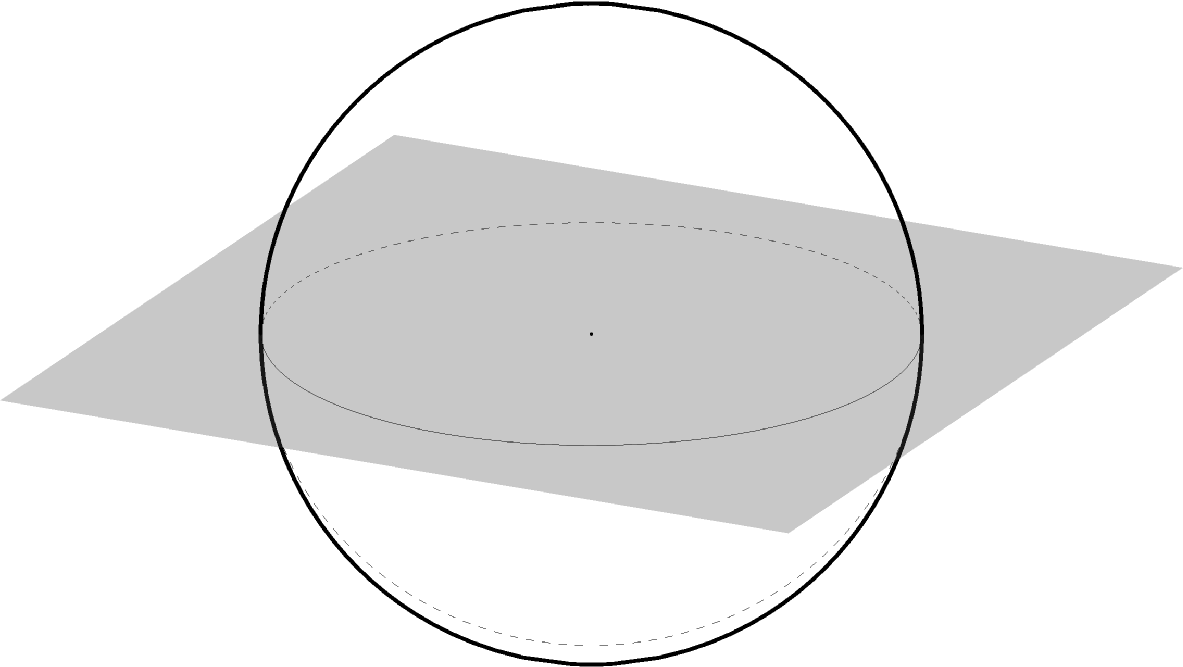
\includegraphics[width=.5\textwidth]{figs/sph-1pl.pdf}
	\caption{A great circle on the sphere with its identifying plane.}
	\label{fig:sphereline}
\end{figure}


In the plane, there is a unique line passing through any two distinct points.  This is almost the case on the sphere, except that we need to exclude one more case.


\begin{observation}
	Given any two points $p$ and $q$ on the sphere which are not antipodal (meaning that our points aren't of the form $p=(x,y,z)$ and $q=(-x,-y,-z)$), there is a unique great circle through $p$ and $q$. 
\end{observation}
\begin{proof}
	To see this, consider the characterization of great circles as the intersections of the surface of the sphere with planes through the center of the sphere.  Since $p$ and $q$ are not antipodes, they are not both collinear with $(0,0,0)$ and so these three points uniquely determine a plane.  This plane intersects the sphere along a great circle which contains $p$ and $q$.
\end{proof}

If $p$ and $q$ \textit{are} antipodal, then any great circle containing one must contain the other as well, so there are infinitely many such great circles.

\begin{figure}[htb]
	\centering
	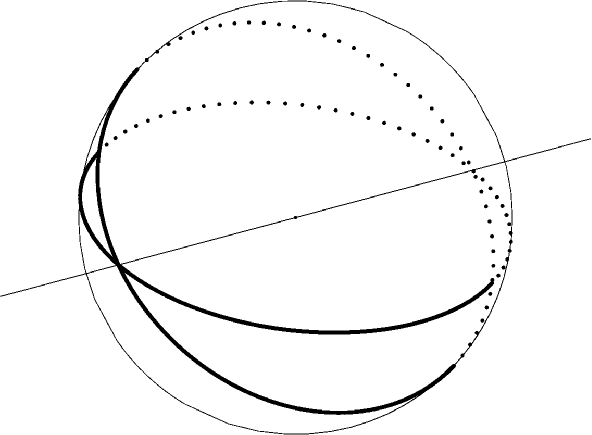
\includegraphics[width=.35\textwidth]{figs/2gc.pdf}
	\caption{Two great circles meet at antipodal points.}
	\label{fig:2gc}
\end{figure}


We now have enough terminology to show a very important fact about spherical geometry.  This  observation is one of the salient features which distinguishes it from the more familiar planar geometry.


\begin{claim}
	Any pair of distinct great circles on the sphere intersect exactly twice, and the points of intersection are antipodes.
\end{claim}
\begin{proof}
	Any two distinct planes determine two distinct great circles, and these planes intersect along a line in $\R^3$ which passes through $(0,0,0)$ and therefore meets the sphere itself at exactly two points, which must be antipodes.
\end{proof}



\zs{the content of this paragraph is important, but the way i've said it is not very clean}
Why is this weird? In the plane, it is always the case that any pair of distinct lines intersects exactly once or they never intersect, in which case we call them \textit{parallel}. Since distinct great circles on the sphere intersect exactly twice, there is no such thing as `parallel lines' on the sphere, and we have to be careful about discussing `the' intersection of two great circles since they do not meet at a unique point.  Furthermore, it is not the case that there is a unique segment of a great circle connecting any two points; there are two, but unless these two points are antipodes, one of the two segments will be shorter.  This shorter segment is the geodesic connecting those points.



We will use this distinction to derive a result which we will use critically in the main theorems of this paper, namely\\

\noindent\textbf{\Cref{lem:sphtri}.}
\emph{The sum of the interior angles of a spherical triangle is strictly greater than $\pi$.  More specifically, the sum of the interior angles is equal to $\pi$ plus the area of the triangle.}

Contrast this to the planar setting, where the sum of the interior angles of a triangle is equal to $\pi$ for any triangle, regardless of its area.  As a concrete example, we can construct a spherical triangle with three right angles.  The triangle formed by the north pole and two points on the equator, one a quarter of the way around the sphere from the other, form such a triangle.  Its area is one eighth of the whole sphere, or $\tfrac{\pi}{2}$, which is, not coincidentally, equal to $\tfrac{\pi}{2}+\tfrac{\pi}{2}+\tfrac{\pi}{2} - \pi$.


In order to  show \Cref{lem:sphtri}, we need some way to translate between \textit{angles} and \textit{area}.  To do that, we'll use a shape which doesn't even exist in the plane: the \textit{diangle} or \textit{lune}.  Consider two distinct great circles.  We know they intersect at two antipodal points, and we can also see that they cut the surface of the sphere into four regions.  Consider one of these regions.  Its boundary is a pair of great circle segments which connect antipodal points and meet at some angle $\theta$ at both of these points.  This shape is a polygon with two sides, hence the name `diangle'.  The term `lune' refers to the crescent moon-shape of this kind of region, and is the term we will use going forward.  \mute{On the Earth, a lune is the region between any two lines of longitude, for example.}

The area of a lune with angle $\theta$ is easy to compute.


\begin{figure}[htb]
	\centering
	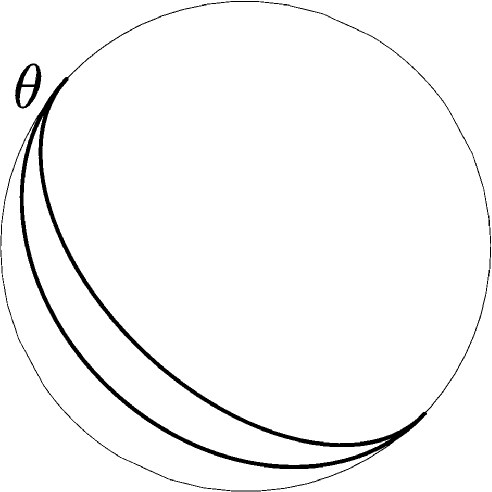
\includegraphics[width=.35\textwidth]{figs/lune.pdf}
	\caption{A lune corresponding to an angle $\theta$. }
	\label{fig:lune}
\end{figure}

\begin{claim}
	Consider a lune whose boundary segments meet at angle $\theta$.  Then the area of this lune is $2\theta$.
\end{claim}
\begin{proof}
	This claim follows from observing that a lune with angle $\theta$ occupies a $\tfrac{2\pi}{\theta}$ portion of the sphere's surface area.  The total surface area of the sphere is $4\pi$, so a lune with angle $\theta$ has surface area $\tfrac{4\pi\theta}{2\pi}= 2\theta$.
\end{proof}

Now that we have a tool that lets us relate angles and areas, we can finally prove the main result of this section.










\begin{lemma}\label{lem:sphtri}
	
	The sum of the interior angles of a spherical triangle is strictly greater than $\pi$.  More specifically, the sum of the interior angles is equal to $\pi$ plus the area of the triangle.
\end{lemma}

\begin{proof}
	Consider a triangle on the sphere with angles $\theta_1$, $\theta_2$, and $\theta_3$.  Let $T$ denote the area of this triangle. If we extend the sides of the triangle to their entire great circles, each pair intersects at the vertices of our triangle as well as the three points antipodal to the vertices of our triangle, and at the same angles at both sets of points.  This triangle is congruent to our triangle, so its area is also $T$.  Each pair of lines cuts the sphere into four lunes, one which contains our triangle, one which contains the antipodal triangle, and two which do not contain either triangle.  We are interested in the three pairs of lunes which do contain the triangles.  We will label these lunes by their angles, so we have a lune $L(\theta_1)$ and its antipodal lune $L'(\theta_1)$, and we can similarly define $L(\theta_2)$, $L'(\theta_2)$, $L(\theta_3)$, and $L'(\theta_3)$.
	
	
	\begin{figure}[htb]
		\centering
		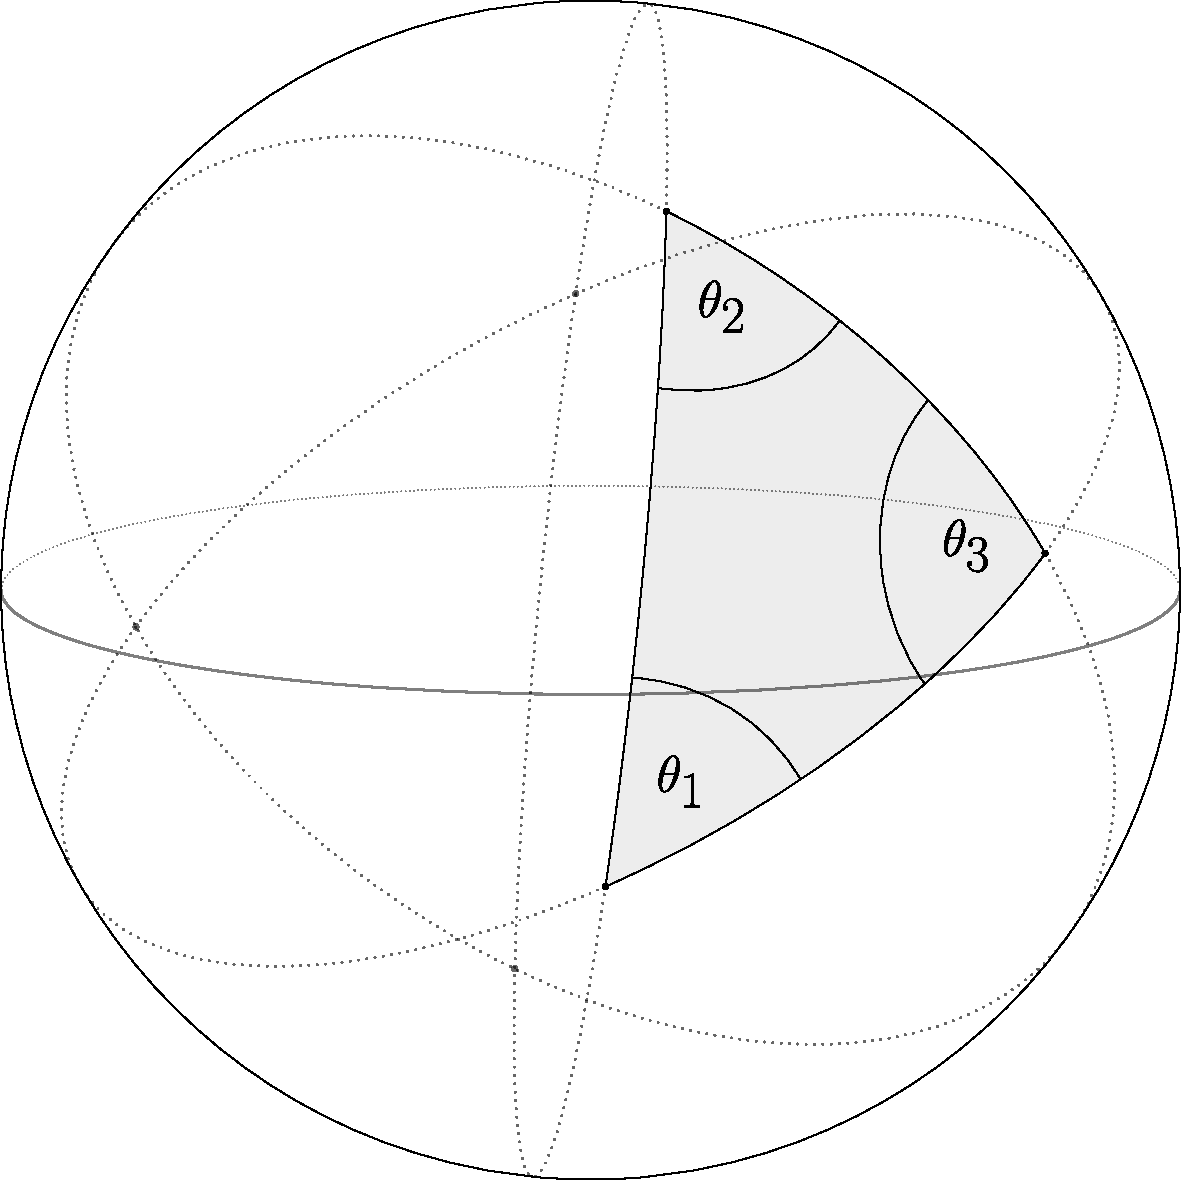
\includegraphics[width=.35\textwidth]{figs/trilune.pdf}
		\caption{A spherical triangle and the antipodal triangle define six lunes.}
		\label{fig:trilune}
	\end{figure}
	
	
	We have six lunes.  In total, they cover the sphere, but share some overlap.  If we remove our triangle from two of the three which contain it and the antipodal triangle from two of the three which contain it, then we have six non-overlapping regions which cover the sphere, so the area of the sphere must be equal to the sum of the areas of these six regions.  We can write
	
	\begin{align*}
	4\pi &= \mathrm{area}(L(\theta_1)) + \mathrm{area}(L'(\theta_1)) \\
	&+  (\mathrm{area}(L(\theta_2)) - T) + (\mathrm{area}(L'(\theta_2)) - T) \\
	&+ (\mathrm{area}(L(\theta_3)) - T)	 + (\mathrm{area}(L'(\theta_3)) - T).
	\end{align*}
	
	And by the earlier claim, we know that the areas of the lunes are twice their angles, so we can rewrite this as
	
	
	\begin{align*}
	4\pi &= 2\theta_1 + 2\theta_1 
	+  (2\theta_2 - T) + (2\theta_2-T) 
	+ (2\theta_3 - T)	 + (2\theta_3 - T)
	\end{align*}
	
	which simplifies to 
	
	\begin{align*}
	\theta_1+\theta_2+\theta_3 = \pi + T,
	\end{align*}
	
	which is exactly the statement we wanted to show.
\end{proof}

We will need one more fact about spherical triangles before we conclude this section.  It dates back to (at least) Euclid's \textit{Elements} \cite{elements} where it follows from Propositions I.6 and I.8.  

\begin{claim}
	An equilateral triangle is equiangular, and vice versa.
\end{claim}

While \textit{Elements} is a compendium of facts about planar geometry, these two propositions do not rely on the assumption that parallel lines exist, and so they hold on the surface of the sphere as well.  
\begin{proof}
	To see this, first suppose that we have a triangle with vertices $a$, $b$, and $c$ and suppose that the length of the side $ab$ is equal to that of $bc$, and let $m$ be the midpoint of the segment $bc$.  Consider the segment $am$. This splits the triangle $abc$ into two triangles $amb$ and $amc$.  These three triangles have the same side lengths and are therefore congruent.  By this congruence, the angle opposite vertex $a$ is equal to the angle opposite vertex $c$.  To show that either of these is also equal to the angle opposite vertex $b$, take $m$ to be the midpoint of segment $ac$.
	
	To see the converse, suppose that the angles at vertices $b$ and $c$ are equal.  Then the triangle $abc$ is congruent to the triangle $acb$ because they both share side $bc$ and the angle at vertex $a$, and the angle at vertex $b$ is equal to that at $c$.\footnote{This is sometimes called the ``side-side-angle'' congruence theorem.}  Since the triangles are congruent, the sides $ac$ and $ab$ have equal length.  To show that either of these is also equal to the length of side $bc$, consider angles $a$ and $c$ instead.
\end{proof}


Now that we have built the necessary tools of spherical geometry, we will wrap up this section with a battery of definitions. 
We carefully lay out these definitions so
as to align with an intuitive understanding of the concepts and to
appease the astute reader who may be concerned with edge cases,
geometric weirdness, and nonmeasurability. 









\begin{definition}
	A \textbf{region} $\Omega$ in $\mathbb{S}^2$ or 
	in $\R^2$ is a non-empty open set together with its
	boundary, such that $\Omega$ is compact and the boundary can be described piecewise as 
	a finite collection of smooth curves.
\end{definition}

This definition is highly technical to allow us to assume away any annoying edge 
cases that might crop up.  Piece-by-piece, a \textit{non-empty open set} lets us 
talk about the \textit{area} of a region in a sensible way. Specifying that a region 
must be \textit{compact} gets rid of cases where we have to worry about regions having 
infinite area.  The entire plane should not be considered a `region'.  Finally, the 
\textit{piecewise-smooth boundary} condition gives us a way to talk about the \textit{perimeter} 
of a region.  We don't want to have to worry about fractal-like shapes which have well-defined 
area but an infinite perimeter or shapes such as a collection of line segments which meet at a point, which has a well-defined perimeter but no area.










\begin{definition}
  A \textbf{compactness score function} $\mathcal{C}$ is a function from
  the set of all regions to the positive real numbers.  We adopt the
  convention that a region with a \textit{higher} compactness score is
  \textit{more} compact, and this naturally induces a partial order over
  the set of all regions, where $A$ is at least as compact as $B$ if and
  only if $\mathcal{C}(A)\geq \mathcal{C}(B)$.
\end{definition}

The final major definition we need is that of a \textit{map
projection}.  In reality, the regions we are interested in comparing
sit on the surface of the Earth (i.e. a sphere), but these regions are
often examined after being projected onto a flat sheet of paper or
computer screen, and so have been subject to such a projection.

\begin{definition}
  A \textbf{map projection} $\varphi$ is a 
  diffeomorphism from a region on the sphere to a region on the 
  plane. 
\end{definition}

Intuitively, a map projection is a well-defined, invertible function between the sphere and the plane which sends regions on the sphere to regions in the plane.  Throughout, we use $\vphi$ to denote such a function from a region of the sphere 
to a region of the plane and $\vphi^{-1}$ its inverse, which goes from a region of the plane to a region of the sphere. 

\begin{definition}
  We use the word \textbf{transformation} [of the plane/sphere] to mean
  to a diffeomorphism from the plane or sphere to itself.
\end{definition}

Since the image of a region under a map projection $\varphi$ is also
a region, we can examine the compactness score of that region both 
before and after applying $\varphi$, and this is the heart of the
problem we address in this paper.  We demonstrate, for several
examples of compactness scores $\mathcal{C}$, that the order
induced by $\mathcal{C}$ is different than the order induced by
$\mathcal{C}\circ\varphi$ for \textit{any} choice of map projection
$\varphi$.

\begin{definition}
  We say that a map projection $\vphi$ \textbf{preserves the  
  compactness score ordering} of a score $\mc{C}$ if for any regions 
  $\Omega,\Omega'$ in the sphere, $\mc{C}(\Omega)\ge \mc{C}(\Omega')$ 
  if and only if $\mc{C}(\vphi(\Omega)) \ge \mc{C}(\vphi(\Omega'))$ in the plane.
\end{definition}

   This is a weaker condition than simply preserving the raw compactness scores. 
   If there is some map projection which results in adding $.1$ to the score of each region, the raw scores are certainly not preserved, but the ordering of regions by their scores is. Additionally, $\vphi$ preserves a compactness score ordering 
  if and only if $\vphi^{-1}$ does.


\zs{this should be moved to the geometry section}
\begin{definition}
  A 
  \textbf{cap} on the sphere  $\mbb{S}^2$ is a region on the sphere
 which can be described as all of the points on the sphere to one side of some plane 
 in $\R^3$.  A cap has a \textit{height}, which is the largest distance between this cutting plane and the cap, and a \textit{radius}, which is the radius of the circle formed by the intersection of the plane and the sphere.  See \Cref{fig:caphr} for an illustration.
\end{definition}


\begin{figure}[h]
  \centering
  %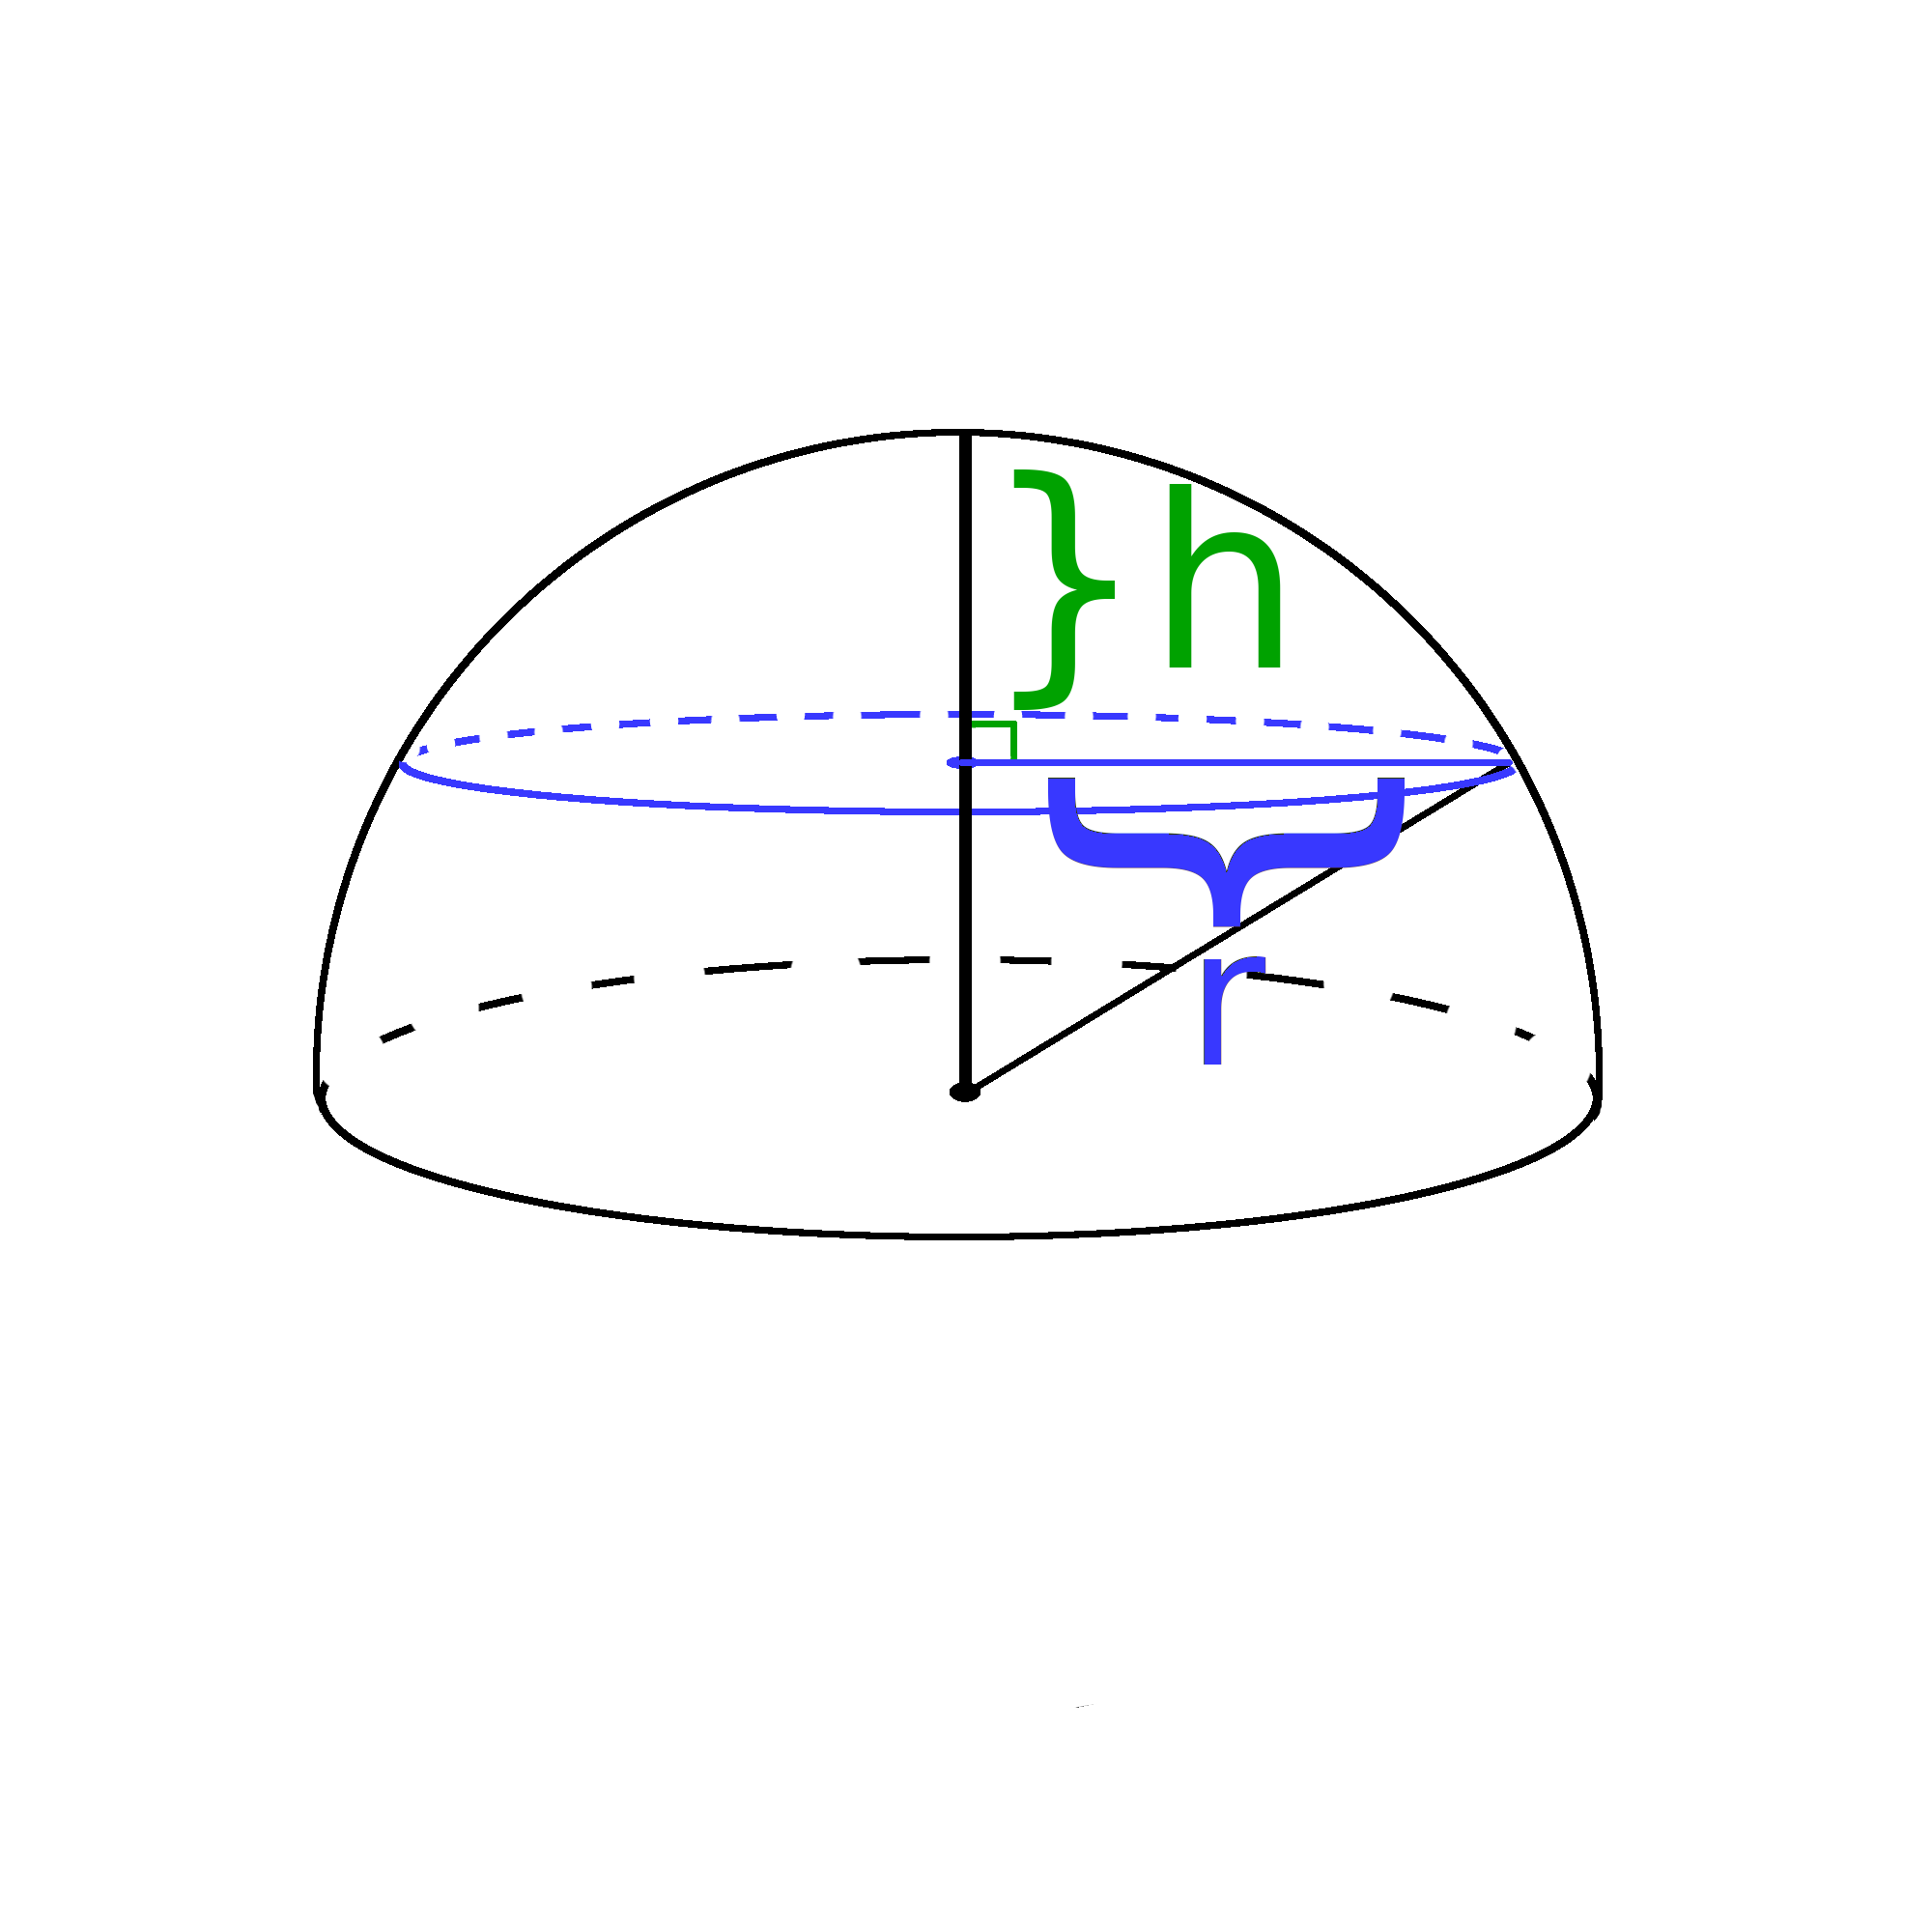
\includegraphics[width=.3\textwidth]{figs/spherecapschema}\\[1.5em]
  \definecolor{qqqqff}{rgb}{0,0,1}

\definecolor{ccqqqq}{rgb}{0.8,0,0}

\definecolor{ududff}{rgb}{0.30196078431372547,0.30196078431372547,1}

\begin{tikzpicture}[line cap=round,line join=round,>=triangle 45,x=1cm,y=1cm]

\clip(-4.493355050909743,-1.2748355780287404) rectangle (4.462150807191927,4.785872976331056);

\draw [shift={(0,0)},line width=3.2pt]  plot[domain=0:3.141592653589793,variable=\t]({1*4*cos(\t r)+0*4*sin(\t r)},{0*4*cos(\t r)+1*4*sin(\t r)});

\draw [shift={(0.0016366799970421299,9.441278259356354)},line width=2pt]  plot[domain=4.286394541961201:5.138764290071874,variable=\t]({1*7.708897306730456*cos(\t r)+0*7.708897306730456*sin(\t r)},{0*7.708897306730456*cos(\t r)+1*7.708897306730456*sin(\t r)});

\draw [shift={(0.019848790872865698,-6.481795867514522)},line width=2pt,dotted]  plot[domain=1.22830273729039:1.9174384984929125,variable=\t]({1*9.441973016351305*cos(\t r)+0*9.441973016351305*sin(\t r)},{0*9.441973016351305*cos(\t r)+1*9.441973016351305*sin(\t r)});

\draw [line width=2pt,color=ccqqqq] (0,2.4033620491027756)-- (0,4);

\draw [line width=2pt,color=qqqqff] (0,2.4033620491027756)-- (3.2001911763834157,2.3997450770024993);

\begin{scriptsize}

\draw [fill=ududff] (0.0016366799970421299,9.441278259356354) circle (2.5pt);

\draw [fill=ududff] (0.019848790872865698,-6.481795867514522) circle (2.5pt);

\draw[color=ccqqqq] (0.26805571312169243,3.3034918797019284) node {\LARGE$h$};

\draw[color=qqqqff] (1.6285727817769453,2.167711482419824) node {\LARGE $r$};

\end{scriptsize}

\end{tikzpicture}
  \caption{ The height $h$ and radius $r$ of a spherical cap. }
  \label{fig:caphr}
\end{figure}






\section{Polsby-Popper}\label{sec:pp}
The final compactness score we analyze is the \textit{Polsby-Popper
score}, which takes the form of an \textit{isoperimetric quotient},
meaning it measures how much area a region's perimeter encloses,
relative to all other regions with the same perimeter.

\begin{definition}\label{def:pp}
  The Polsby-Popper score of a region $\Omega$ is defined to be
  $$\mathrm{PP}(\Omega) = \frac{4\pi
  \cdot\mathrm{area}(\Omega)}{\mathrm{perim}(\Omega)^2}$$ 
in either the sphere or the plane, and
  $\mathrm{area}$ and $\mathrm{perim}$ are the area and perimeter of
    $\Omega$, respectively.
\end{definition}

The ancient Greeks were first to observe that if $\Omega$ is a region
in the plane, then $4\pi\cdot\mathrm{area}(\Omega)\leq
\mathrm{perim}(\Omega)^2$, with equality if and only if $\Omega$ is
a circle. This became known as the \textit{isoperimetric inequality} in
the plane.  This means that, in the plane, $0\le \mathrm{PP}(\Omega)\le 1$,
where the Polsby-Popper score is equal to $1$ only in the case of
a circle. We can observe that the Polsby-Popper score is scale-invariant in
the plane. 

An isoperimetric inequality for the sphere exists, and we
state it as the following lemma.  For a more detailed treatment of
isoperimetry in general, see \cite{osserman1979bonnesen}, and for
a proof of this inequality for the sphere, see \cite{rado}.

\begin{lemma}
  If $\Omega$ is a region on the sphere with area
  $A$ and perimeter $P$, then $P^2\geq A^2-4\pi A$ with equality if
  and only if $\Omega$ is a spherical cap.
\end{lemma}
A consequence of this is that among all regions on the sphere with
a fixed area $A$, a spherical cap with area $A$ has the shortest
perimeter. However, the key difference between the isoperimetric 
quotient in the plane and on the sphere is that on the 
sphere, there is no scale invariance.


\begin{lemma}\label{lem:ppscale}
  Let $S$ be the unit sphere, and let $\kappa(h)$ be a cap of height
  $h$.  Then $\mathrm{PP}(\kappa(h))$ is
  a monotonically increasing function of $h$.
\end{lemma}


\begin{proof}
  Let $r(h)$ be the radius of the circle bounding $\kappa(h)$. We
  compute: 
  \begin{align*}
    1 &= r(h)^2 + (1-h)^2 \text {, by right triangle trigonometry}\\ 
      &= r(h)^2 + 1 - 2h+h^2
  \end{align*}
  Rearranging, we get that $r(h)^2= 2h-h^2$, which we can plug in to
  the standard formula for perimeter:
  \begin{align*}
    \mathrm{perim}_S(\kappa(h)) = 2\pi r(h) = 2\pi \sqrt{2h-h^2}
  \end{align*}
  We can now use the Archimedian equal-area projection 
  defined by $(x,y,z) \to
  \left(\frac{x}{\sqrt{x^2+y^2}},\frac{y}{\sqrt{x^2+y^2}}, z\right)$ 
  to compute $\mathrm{area}_S(\kappa(h)) = 2\pi h$ and plug it in to 
  get:

  \begin{align*}
    \mathrm{PP}_S(\kappa(h)) = \frac{4\pi (2\pi h) }{4 \pi^2 (2h-h^2)}
    = \frac{2}{2-h}
  \end{align*}
  Which is a monotonically increasing function of $h$.
\end{proof}
\begin{corollary}\label{cor:capscale}
  On the sphere, Polsby-Popper scores of caps are monotonically
  increasing with area
\end{corollary}
Using this, we can show the main theorem of this section, that no map
projection from a region on the sphere to the plane can preserve the ordering
of Polsby-Popper scores for all regions.  

\begin{theorem}\label{thm:dpp}
  If $\varphi:U\to V$ is a map projection from the sphere to the plane,
  then there exist two regions $A,B\subset U$ such that
  the Polsby-Popper score of $B$ is greater than that of $A$ in the
  sphere, but the Polsby-Popper score of $\varphi(A)$ is greater than
  that of $\varphi(B)$ in the plane.
\end{theorem}
\begin{figure}[h]\label{fig:dpp}
  \centering
  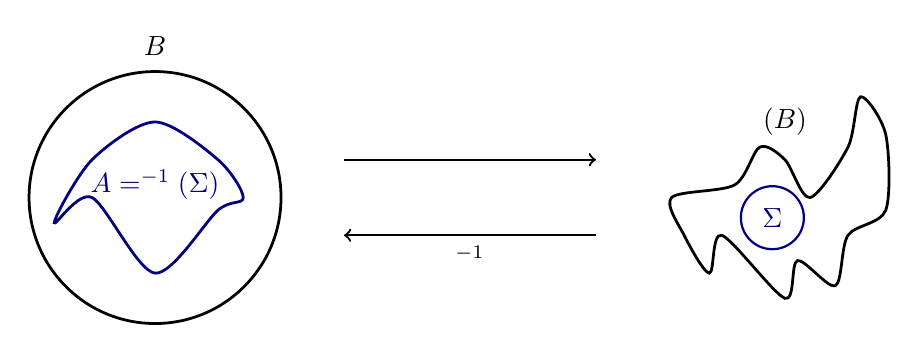
\begin{tikzpicture}[scale=1.6]
    \draw[thick,->] (-1,0.3)-- (1,0.3)%
    node[midway,above] {$\vphi$};
    \draw[thick,->] (1,-0.3) -- (-1,-0.3)%
    node[midway,below] {$\vphi^{-1}$}; 
    \draw[line width=1, black] (-2.5,0) circle (1);
    \draw node at (-2.5,1.2) {\color{black} $B$};
    \draw[line width=1, black] plot [smooth cycle, tension=0.5]%
    coordinates { (2.5,-0.8) (2.6,-0.5) (2.9,-0.7) (3,-0.3) (3.3,-0.1)% 
    (3.3,0.5) (3.1,0.8) (3,0.4) (2.7,0) (2.5,0.3) (2.3,0.4)%
    (2.1,0.1) (1.6,0) (1.7,-0.3) (1.9, -0.6) (2,-0.3)};
    \draw node at (2.5,0.6) {\color{black} $\vphi(B)$};

    \draw[thick, NavyBlue] (2.4,-0.16) circle (0.25);
    \draw node at (2.4,-0.16) {\color{NavyBlue} $\Sigma$};
    \draw[line width=1, NavyBlue] plot [smooth cycle, tension=0.5]%
    coordinates { (-2.5,-0.6) (-3, 0) (-3.3,-0.2) (-3,0.3) (-2.5,0.6)%
    (-2,0.3) (-1.8,0) (-2,-0.1)};
    \draw node at (-2.5,0.1) {\color{NavyBlue} $A=\vphi^{-1}(\Sigma)$};
  \end{tikzpicture}
  \caption{The construction of regions $A$, $B$, and $\hat{A}$ in the
  proof of Theorem~\ref{thm:dpp}.} 
\end{figure}

\begin{proof}
  Let $\varphi$ be a map projection, and let 
  $\kappa \subset U$ be some cap. We will take our regions 
  $A$ and $B$ to lie in $\kappa$. Set $B$ to be a cap 
  contained in $\kappa$. Let $\Sigma$ be a circle in 
  the plane such that $\Sigma
  \subsetneq \varphi(B)$ and let $A=\varphi^{-1}(\Sigma)$ (see
  Figure~\ref{fig:dpp}).

  We now use the isoperimetric inequality for the sphere 
  and Corollary~\ref{cor:capscale} to claim that 
  $A$ does not maximilze Polsby-Popper score in the sphere.

  To see this, take $\hat{A}$ to be a cap in the sphere with 
  area equal to that of $A$. Note that since the 
  area of $\hat {A}$ is less than the area of the cap $B$, it 
  follows that we can choose $\hat{A}\subset B$. 
  
  By the isoperimetric inequality of the sphere, 
  $\mathrm{PP}_S(\hat{A})\geq
  \mathrm{PP}_S(A)$. Since map projections preserve containment,
  $\Sigma\subsetneq \varphi(B)$ implies that $A\subsetneq B$, 
  meaning that $\mathrm{area}(\hat A) = \mathrm{area}(A)\lneq 
  \mathrm{area}(B)$. By Corollary~\ref{cor:capscale}, we know that
  $\mathrm{PP_S}(\hat{A})< \mathrm{PP_S}(B)$, and combining this with
  the earlier inequality, we get
  \begin{align*}
    \mathrm{PP_S}({A})\leq \mathrm{PP_S}(\hat{A})< \mathrm{PP_S}(B)
  \end{align*}

  Since $\Sigma = \varphi(A)$ maximizes the Polsby-Popper score in the
  plane, but $A$ does not do so in the sphere, we have shown that
  $\varphi$ does not preserve the maximal elements in the score
  ordering, and therefore it cannot preserve the ordering itself.
\end{proof}

The reason why every map projection fails to preserve the ordering of
Polsby-Popper scores is because the score itself is constructed from
the \textit{planar} notion of isoperimetry, and there is no reason to
expect this formula to move nicely back and forth between the sphere
and the plane.  This proof crucially exploits a scale invariance
present in the plane but not the sphere.  If we consider any circle in
the plane, it's Polsby-Popper score is definitionally equal to one,
but that is not true of every cap in the sphere.  \mute{This naturally
raises the question of whether being more careful, and defining
a compactness score which uses the isoperimetric quotient of the
surface the region is actually in will evade this problem.  We show
later that it does resolve the issue of scale-noninvariance, but it is
still induces an ordering which is not preserved by any map
projection.  We discuss this further in \Cref{sec:generalz}.}

\section{Convex Hull}\label{sec:ch}
We first consider the \textit{convex hull
score}.  We briefly recall the definition of a convex set and then
define this score function.
\zs{add discussion about the use of this score, why it's good, why not}


\begin{definition}
	A set in a metric space is \textbf{convex} if every shortest geodesic segment between any two points in the set is entirely 
	contained within that set.
\end{definition}





\begin{definition}
  Let $\mathrm{conv}(\Omega)$ denote the \textit{convex hull} of
  a region $\Omega$ in either the sphere or the plane, which is the
  smallest convex region containing $\Omega$.  Then we define the
  \textit{convex hull score} of $\Omega$ as 
  \begin{align*}
    \mathrm{CH}(\Omega)=
    \frac{\mathrm{area}(\Omega)}{\mathrm{area}(\mathrm{conv}(\Omega)).}
  \end{align*}
  
  Since the intersection of convex sets is a convex set, there is a unique smallest (by area) convex hull for any region $\Omega$.
\end{definition}



\begin{figure}[htb]
	\centering
	%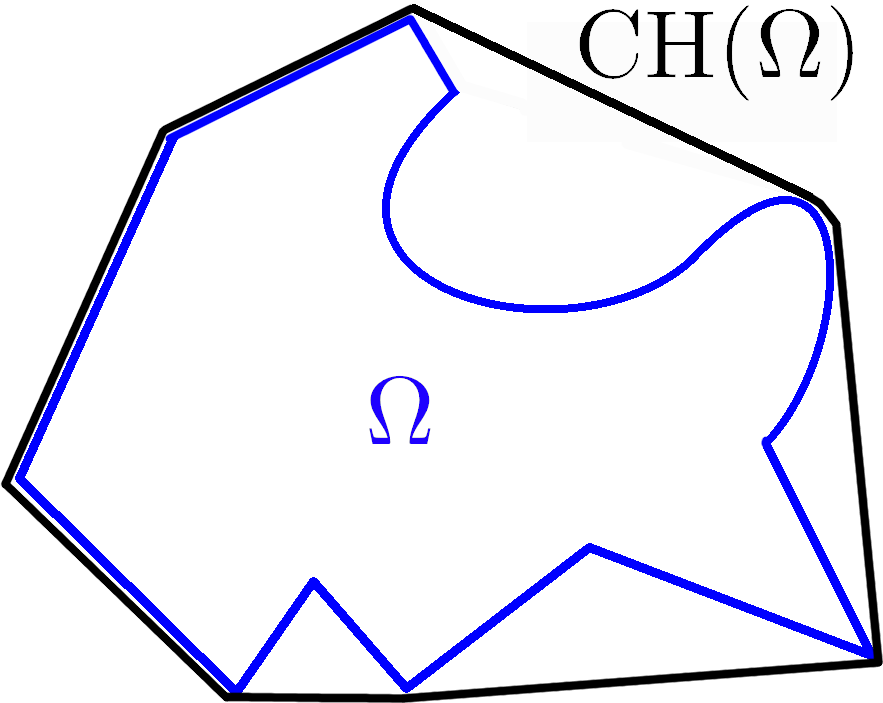
\includegraphics[width=.35\textwidth]{figs/ch_example.png}
	
\definecolor{qqqqff}{rgb}{0,0,1}
\begin{tikzpicture}[scale=1.5,line cap=round,line join=round,>=triangle 45,x=1cm,y=1cm]
\clip(-3.1808855374298814,0.7054196919809391) rectangle (2.8436799719688346,4.78259146738453);
\draw [line width=2pt,color=qqqqff] (-0.5403387932320529,4.199917026631047)-- (-1.4876311065851997,3.283901898015972);
\draw [line width=2pt,color=qqqqff] (-2.59555742277687,2.1884264530340003)-- (-1.030093019846988,1.0427513872026393);
\draw [line width=2pt,color=qqqqff] (-1.030093019846988,1.0427513872026393)-- (-0.4266458477678716,2.503268455857886);
\draw [line width=2pt,color=qqqqff] (-0.4266458477678716,2.503268455857886)-- (1.1213273327829054,2.310865009687734);
\draw [line width=2pt,color=qqqqff] (1.1213273327829054,2.310865009687734)-- (0.6315731061679702,3.8850750238071616);
\draw [shift={(-2.4623421270336228,3.1638741521373337)},line width=2pt,color=qqqqff]  plot[domain=-1.7065250247888804:0.12252504290266225,variable=\t]({1*0.9845021730326186*cos(\t r)+0*0.9845021730326186*sin(\t r)},{0*0.9845021730326186*cos(\t r)+1*0.9845021730326186*sin(\t r)});
\draw [shift={(-0.01568921678809781,3.814254744830714)},line width=2pt,color=qqqqff]  plot[domain=0.10898159374480773:2.5077053734556625,variable=\t]({1*0.6511252004282949*cos(\t r)+0*0.6511252004282949*sin(\t r)},{0*0.6511252004282949*cos(\t r)+1*0.6511252004282949*sin(\t r)});
\draw [line width=2.8pt] (-2.685655712545722,2.2031756923666004)-- (-1.0153159792750968,0.9768503185729869);
\draw [line width=2.8pt] (-1.0153159792750968,0.9768503185729869)-- (1.158637184087576,2.29171136125267);
\draw [line width=2.8pt] (1.158637184087576,2.29171136125267)-- (0.6620716009713541,4.04266375305702);
\draw [shift={(-0.01540854579167931,3.8076224532316205)},line width=2.8pt]  plot[domain=0.33394133978769747:2.3774678762164125,variable=\t]({1*0.7170939700497241*cos(\t r)+0*0.7170939700497241*sin(\t r)},{0*0.7170939700497241*cos(\t r)+1*0.7170939700497241*sin(\t r)});
\draw [line width=2.8pt] (-2.685655712545722,2.2031756923666004)-- (-0.5331419341269765,4.30378361705294);
\draw [color=qqqqff](-0.7863560820341027,3.2000351515748306) node[anchor=north west] {\LARGE$\Omega$};
\draw (0.1549822788094467,1.5938421717062845) node[anchor=north west] {\LARGE$\mathrm{CH}(\Omega{)}$};
\end{tikzpicture}

	\caption{A region $\Omega$ and its convex hull.}
	\label{fig:ch_example}
\end{figure}

Suppose that our map projection $\vphi$ does  preserve the ordering of regions under the convex hull scores of all regions in a patch on the sphere and a patch in the plane.  We begin by observing that such a projection must preserve certain geometric properties of regions within these patches.
\begin{lemma}~\label{lem:CH_prep}
	If $\vphi$ preserves the ordering of regions induced by their convex hull scores, then the following must 
	hold:
	\begin{enumerate}
		\item $\vphi$ and $\vphi^{-1}$ send convex regions to convex regions
		\item $\vphi$ sends every segment of a great circle on the sphere to a line segment in the plane.  That is, it preserves geodesics.
		\item There exists a region $U$ in the domain of $\vphi$
		such that for any regions $A,B\subset U$, if 
		$A$ and $B$ have equal area on the sphere, then 
		$\vphi(A)$ and $\vphi(B)$ have equal area in the plane.  The same holds 
		for $\vphi^{-1}$ for all pairs of regions inside of $\vphi(U)$.
	\end{enumerate}
\end{lemma}

\begin{figure}[h]
	\centering
	%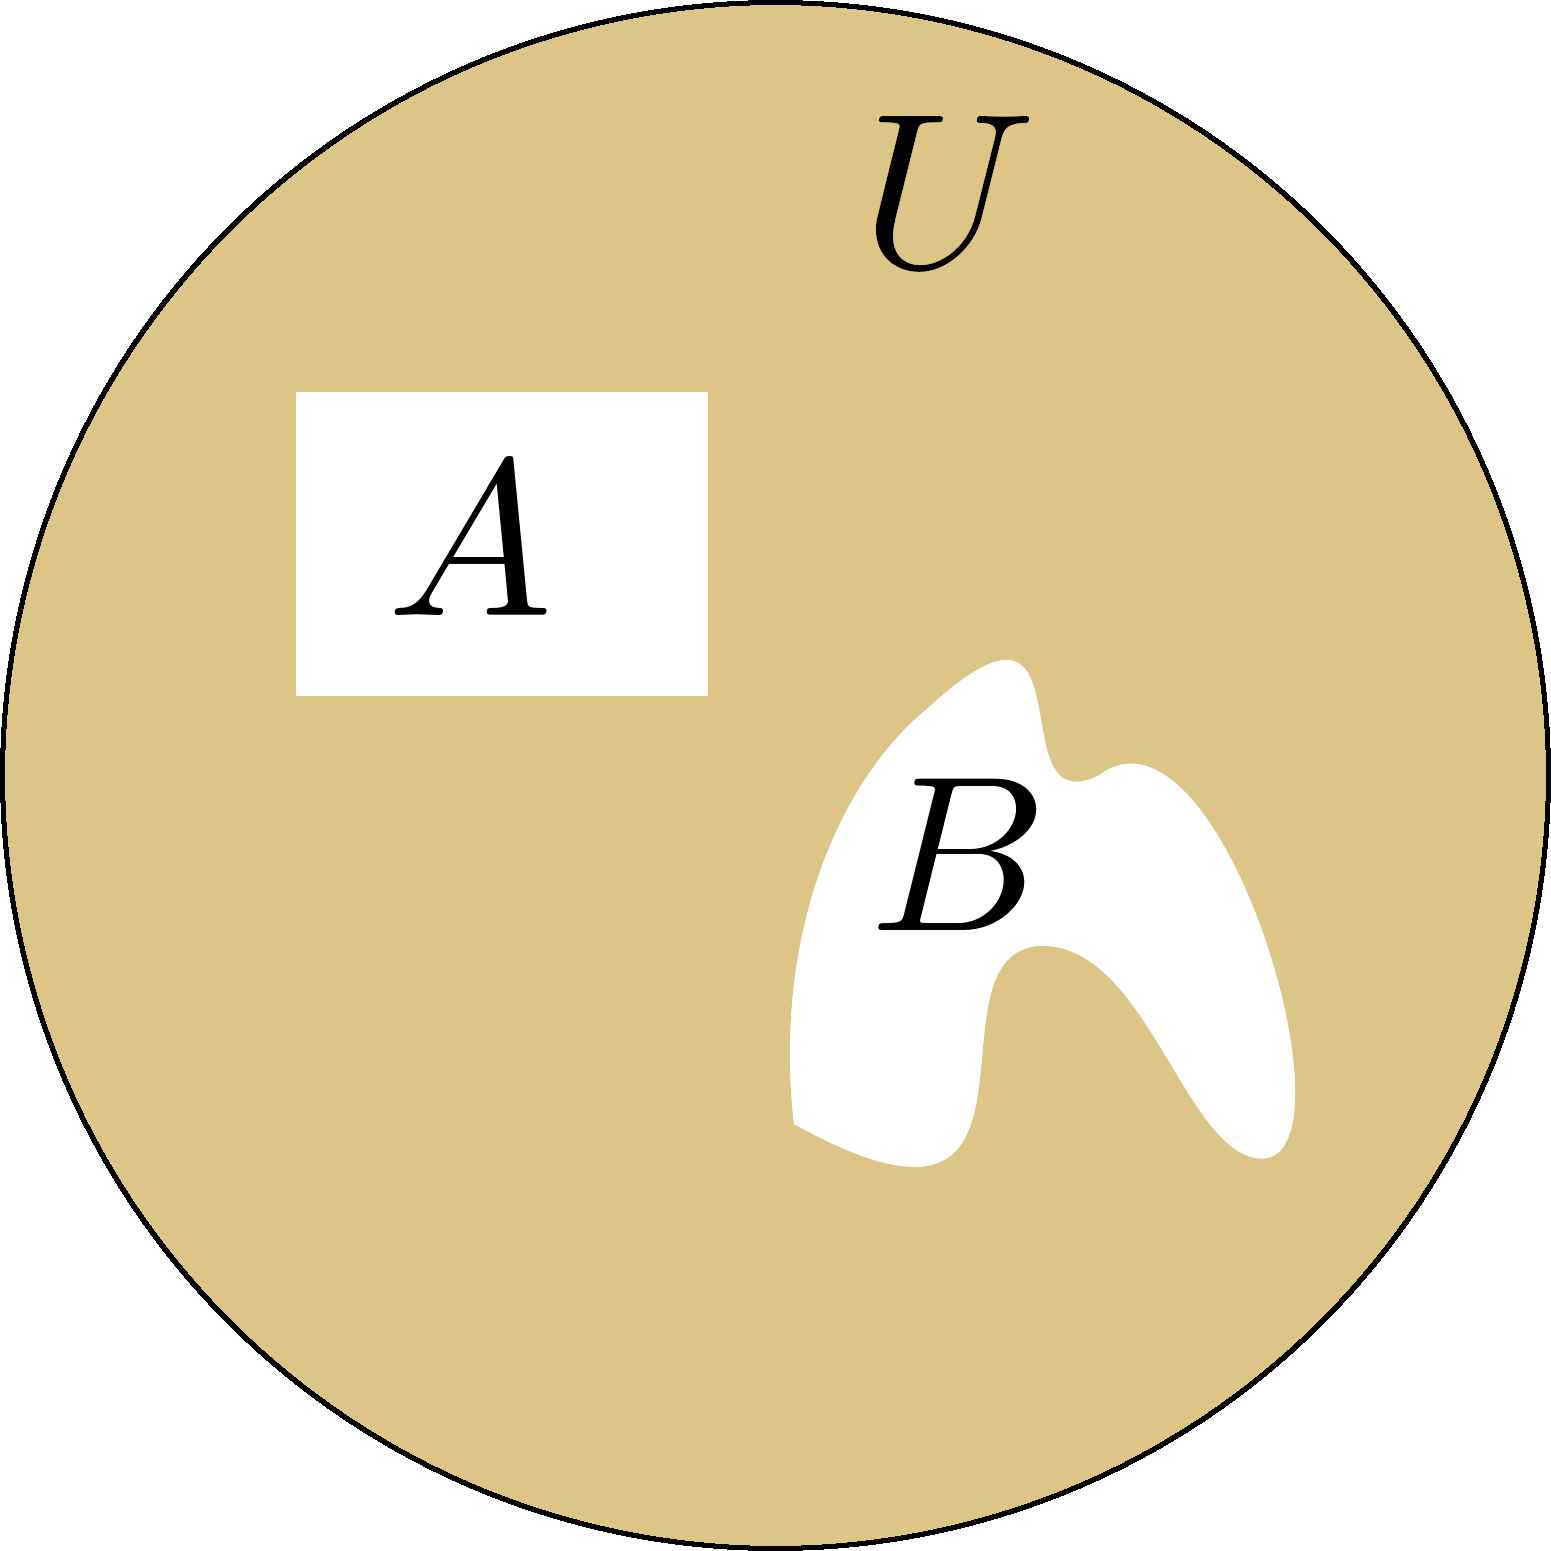
\includegraphics[width=.25\textwidth]{figs/ch_sphere_schema.png}
	\definecolor{ffffff}{rgb}{1,1,1}


\begin{tikzpicture}[scale=.35,line cap=round,line join=round,>=triangle 45,x=1cm,y=1cm]

\clip(-6.762534270657285,-7.4038512549636435) rectangle (12.125044594505917,5.378465301245481);
\draw [line width=3.6pt,fill=black,fill opacity=0.27] (2.52,-1.24) circle (5.094349811310566cm);
\draw [line width=0.4pt,color=ffffff,fill=ffffff,fill opacity=1] (2.82,-2.62) circle (1.352035502492446cm);
\draw [rotate around={-134.1620339448981:(0.25635345523487,0.2782885419108182)},line width=0.4pt,color=ffffff,fill=ffffff,fill opacity=1] (0.25635345523487,0.2782885419108182) ellipse (1.6381871321999442cm and 0.5964014274522406cm);
\draw [rotate around={2.00955381302114:(1.84,1.24)},line width=0.4pt,color=ffffff,fill=ffffff,fill opacity=1] (1.84,1.24) ellipse (1.2329931677283157cm and 0.46805144125908144cm);
\draw (-0.14942211242749375,1.2652523257265278) node[anchor=north west] {\LARGE$A$};
\draw (2.089030655746763,-1.9839442053140297) node[anchor=north west] {\LARGE$B$};
\draw (5.613994458370557,4.161101819701755) node[anchor=north west] {\LARGE$U$};
\end{tikzpicture}
	\caption{Two equal area regions $A$ and $B$ removed from $U$.}
	\label{fig:ch_schema}
\end{figure}



\begin{proof}
	\ \\
	
	\vspace*{-2em}
	\begin{enumerate}
		\item[] The proof of (1) follows from the idea that any projection which preserves the convex hull score ordering of regions must 
		preserve the maximizers in that ordering.   Here, the maximizers are convex sets.
		
		\item[]  Suppose, for the sake of contradiction, that there is some geodesic segment $s$ on the sphere such that $\vphi(s)$ is not a line segment. Construct two convex spherical polygons $L$ and $M$ which both have $s$ as a side. 
		
		
\begin{figure}[h]
	\centering
	%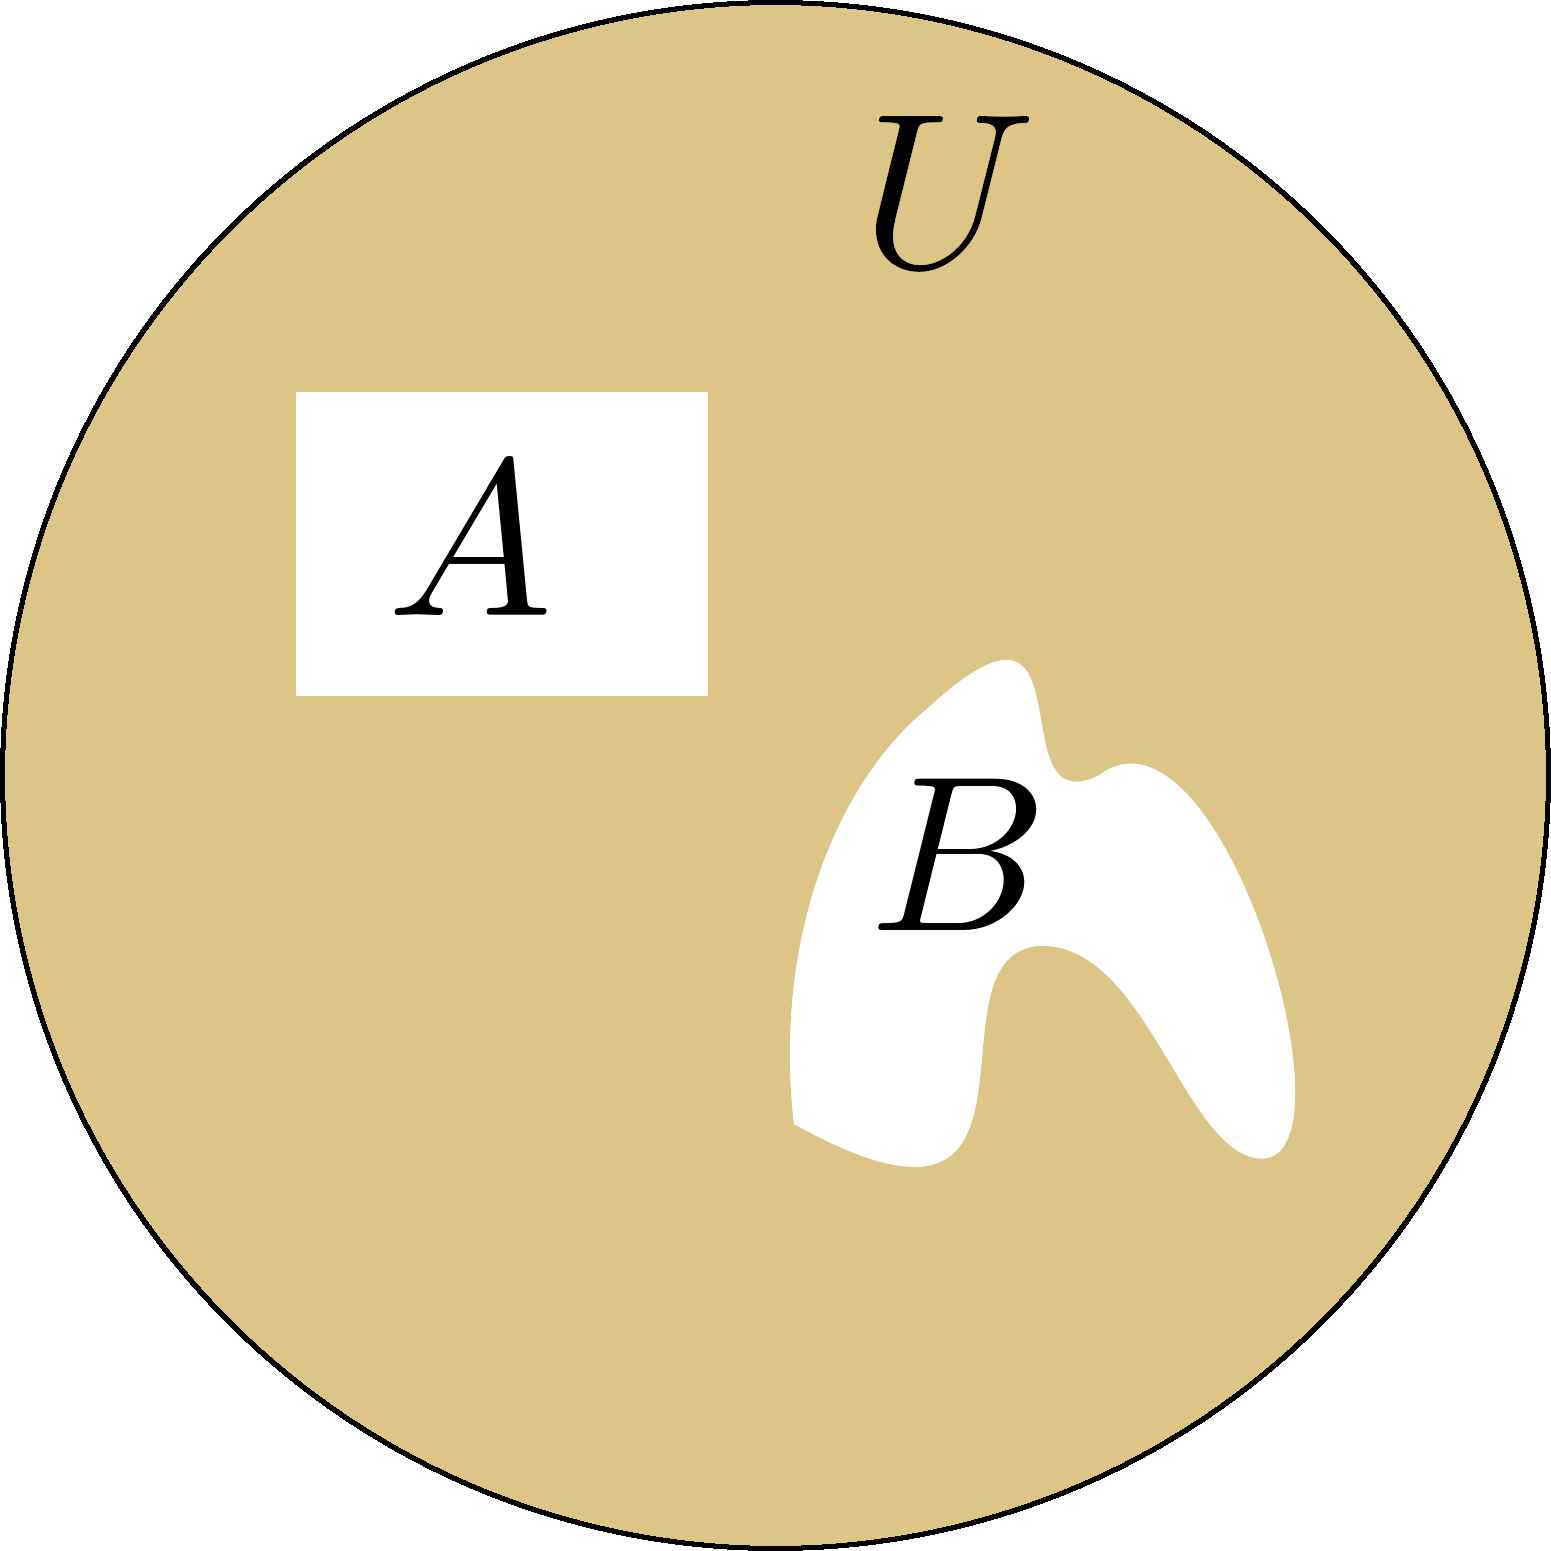
\includegraphics[width=.25\textwidth]{figs/ch_sphere_schema.png}
	
\begin{tikzpicture}[scale=.7,line cap=round,line join=round,>=triangle 45,x=1cm,y=1cm]

\clip(-9.2605723047488,4.939165952768963) rectangle (5.35451137900598,13.039739619301336);
\draw [line width=2pt] (-2.0244628099173525,12.456528925619821)-- (-5.578181818181814,9.216859504132223);
\draw [line width=2pt] (-5.578181818181814,9.216859504132223)-- (-2.338512396694217,5.663140495867761);
\draw [line width=2pt] (-2.338512396694217,5.663140495867761)-- (1.2152066115702453,8.90280991735536);
\draw [line width=2pt] (1.2152066115702453,8.90280991735536)-- (-2.0244628099173525,12.456528925619821);
\draw [shift={(4.190413223140495,8.754049586776851)},line width=2pt]  plot[domain=2.604307939289022:3.5793780144036975,variable=\t]({1*7.234157681502106*cos(\t r)+0*7.234157681502106*sin(\t r)},{0*7.234157681502106*cos(\t r)+1*7.234157681502106*sin(\t r)});
\draw [line width=2pt,color=NavyBlue] (-2.601747508322699,11.243947166759868)-- (-2.9355456436406637,7.507555467344712);
\draw (-4.988752951588037,9.58982716176266) node[anchor=north west] {\LARGE$\varphi(L)$};
\draw (-2.588752951588037,11.42982716176266) node[color=NavyBlue,anchor=north west] {\LARGE$\varphi(s)$};

\draw (-1.9481756813548882,9.58982716176266) node[anchor=north west] {\LARGE$\varphi(M)$};
\begin{scriptsize}
\draw [fill=NavyBlue] (-2.601747508322699,11.243947166759868) circle (2.5pt);
\draw [fill=NavyBlue] (-2.9355456436406637,7.507555467344712) circle (2.5pt);
\end{scriptsize}
\end{tikzpicture}
	\caption{If $\vphi(s)$ is not a line segment, then one of $\vphi(M)$ or $\vphi(L)$ is not convex.}
	\label{fig:lineconvexcont}
\end{figure}
		
		 By (1), $\vphi$ must send both of these polygons to convex regions in the plane, but this is not the case.  All of the points along $\vphi(s)$ belong to both $\vphi(L)$ and $\vphi(M)$, but since $\vphi(s)$ is not a line segment, we can find two points along it which are joined by some line segment which contains points which only belong to $\vphi(L)$ or $\vphi(M)$, which means that at least one of these convex spherical polygons is sent to something non-convex in the plane, which contradicts our assumption.		See \Cref{fig:lineconvexcont} for an illustration.
		
		That $\vphi^{-1}$ sends line segments in the plane to great circle segments on the sphere is shown analogously.  
		
		This completes the proof of (2).
		
		
		
\item[] To show (3), let our region $U$ be a cap, without loss of generality.  Take $A,B$ to be regions of equal area such that $A$ and $B$ are properly contained in the interior of $U$, as in \Cref{fig:ch_schema}.  Define two new regions $X=U\ssm A$ and $Y=U\ssm B$, i.e. these regions are equal to $U$ with $A$ or $B$ deleted, respectively.  

The cap $U$ is itself the convex hull of both $X$ and $Y$, and since $A$ and $B$ have equal area, we have that $\mathrm{CH}(X) = \mathrm{CH}(Y)$.  Since $U$ is a cap, it is convex, so by (1), $\vphi(U)$ is also convex.  Since $\vphi$ preserves the ordering of convex hull scores and $X$ and $Y$ had equal scores on the sphere, $\vphi$ must send $X$ and $Y$ to regions in the plane which also have the same convex hull score.  Furthermore, the convex hulls of $\vphi(X)$ and $\vphi(Y)$ are $\vphi(U)$.

By definition, we have
\begin{align*}
\mathrm{CH}(X) &= \mathrm{CH}(Y)\\
\frac{\mathrm{Area}(\vphi(X))}{\mathrm{Area}(\vphi(U))} &= \frac{\mathrm{Area}(\vphi(Y))}{\mathrm{Area}(\vphi(U))}
\end{align*}
and by the construction of $X$ and $Y$, we have 
\begin{align*}
\frac{\mathrm{Area}(\vphi(U)) - \mathrm{Area}(\vphi(A))}{\mathrm{Area}(\vphi(U))} &= \frac{\mathrm{Area}(\vphi(U)) - \mathrm{Area}(\vphi(B))}{\mathrm{Area}(\vphi(U))}\\
\mathrm{Area}(\vphi(A)) &= \mathrm{Area}(\vphi(B))
\end{align*}
 which is what we wanted to show.  The proof that $\vphi^{-1}$ also has this property is analogous.  This proves (3).
\end{enumerate}
\end{proof}

We can now show that no map projection can preserve the convex hull score ordering of regions by demonstrating that there is no projection from a patch on the sphere to the plane which has all three of the properties described  in \Cref{lem:CH_prep}. 


\begin{theorem}
	There does not exist a map projection with the three properties in Lemma~\ref{lem:CH_prep}
\end{theorem}
\begin{proof}
	Assume that such a map, $\vphi$, exists, and restrict 
	it to $U$ as above. Let $T\subset U$ be a 
	small equilateral spherical  triangle with centered at 
	the center of $U$. Let $T_1$ and $T_2$ be two 
	congruent triangles meeting at a point and 
	each sharing a face with $T$, as in \Cref{fig:sphtris}.

\begin{figure}[!htb]
	\centering
	%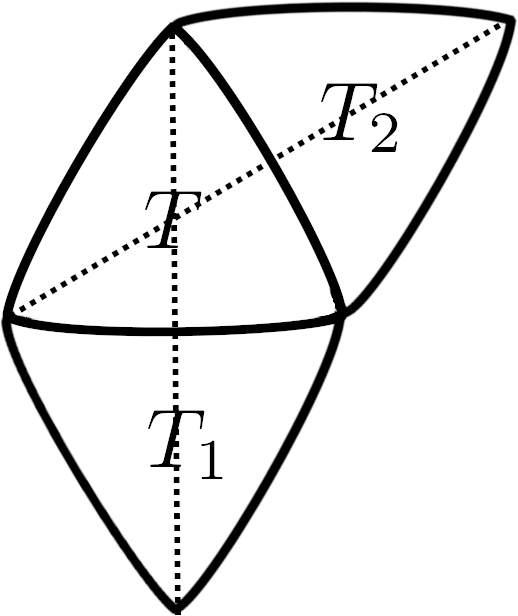
\includegraphics[width=.25\textwidth]{figs/spheretri.png}
	\begin{tikzpicture}[scale=.25,line cap=round,line join=round,>=triangle 45,x=1cm,y=1cm]
\clip(-7.699047690559778,-7.571555155097503) rectangle (6.4348506610533125,7.774557106234026);
\draw [shift={(-1.6505275214910575,9.115278552365504)},line width=2pt]  plot[domain=4.3817706171001:5.059138387806136,variable=\t]({1*10.321001528275485*cos(\t r)+0*10.321001528275485*sin(\t r)},{0*10.321001528275485*cos(\t r)+1*10.321001528275485*sin(\t r)});
\draw [shift={(-10.803070399796216,-4.420666087580098)},line width=2pt]  plot[domain=0.2938195101807776:0.8077763069010403,variable=\t]({1*13.226440769305302*cos(\t r)+0*13.226440769305302*sin(\t r)},{0*13.226440769305302*cos(\t r)+1*13.226440769305302*sin(\t r)});
\draw [shift={(8.343628495049057,-4.490800515766344)},line width=2pt]  plot[domain=2.3753688206179033:2.8611250423804107,variable=\t]({1*13.887257489360788*cos(\t r)+0*13.887257489360788*sin(\t r)},{0*13.887257489360788*cos(\t r)+1*13.887257489360788*sin(\t r)});
\draw [shift={(-7.513162654544307,7.579158955824589)},line width=2pt]  plot[domain=5.566336287533996:6.169114070716076,variable=\t]({1*12.436992398719607*cos(\t r)+0*12.436992398719607*sin(\t r)},{0*12.436992398719607*cos(\t r)+1*12.436992398719607*sin(\t r)});
\draw [shift={(3.7978267211845975,-8.419128622621312)},line width=2pt]  plot[domain=1.4994026026391953:1.954080474540578,variable=\t]({1*14.614520953612525*cos(\t r)+0*14.614520953612525*sin(\t r)},{0*14.614520953612525*cos(\t r)+1*14.614520953612525*sin(\t r)});
\draw [shift={(10.390041391475169,4.172878076060955)},line width=2pt]  plot[domain=3.4450650540010272:3.881445927448308,variable=\t]({1*16.127936863518837*cos(\t r)+0*16.127936863518837*sin(\t r)},{0*16.127936863518837*cos(\t r)+1*16.127936863518837*sin(\t r)});
\draw [shift={(-9.037074369684714,1.4207160457879888)},line width=2pt]  plot[domain=5.463306638850501:6.100385463261517,variable=\t]({1*11.066136404446647*cos(\t r)+0*11.066136404446647*sin(\t r)},{0*11.066136404446647*cos(\t r)+1*11.066136404446647*sin(\t r)});
\draw [line width=1.2pt,dotted,opacity=.3] (4.8403256579539065,6.1581625753487135)-- (-5.001005706626561,-0.6467585545910133);
\draw [line width=1.2pt,dotted,opacity=.3] (-1.613022483529527,5.156840351541236)-- (-1.4587194302885766,-6.643272504200754);
\draw (-1.7868492266322078,1.7623586423065475) node[anchor=north west] {\large$T$};
\draw (-1.8511013622691343,-2.593740589657192) node[anchor=north west] {\large$T_1$};
\draw (1.458165010947301,4.1125782470569596) node[anchor=north west] {\large$T_2$};
\end{tikzpicture}
	\caption{The spherical regions $T,T_1,T_2$.}
	\label{fig:sphtris}
\end{figure}












We first argue that the images of $T\cup T_1$ and $T\cup T_2$ are parallelograms.

Without loss of generality, consider $T\cup T_1$.  By construction, it is a 
convex spherical quadrilateral. By symmetry, its geodesic 
diagonals on the sphere divide it into four triangles of equal area, since the long diagonal splits $T$ and $T_1$ in 
half, and $T$ and $T_1$ have the same area.


		Since $\vphi$ sends spherical geodesics to line segments in the plane, it must send 
		$T\cup T_1$ to a Euclidean quadrilateral $Q$ whose diagonals 
		are the images of the diagonals of the spherical quadrilateral $T\cup T_1$.
		
		 Since 
		$\vphi$ sends equal area regions to equal area 
		regions, it follows that the diagonals 
		of $Q$ split it into four equal area triangles.
		
		We now argue that this implies that $Q$ is a Euclidean parallelogram by showing that its diagonals bisect each other.  Since the four triangles 
		formed by the diagonals of $Q$ are all the same area, we can pick two of these triangles which share a side 
		and consider the larger triangle formed by their union.  One side of this triangle is a diagonal $d_1$ of $Q$ and its area is 
		bisected by the other diagonal $d_2$, which passes through $d_1$ and its opposite vertex.  This area bisector passes through the midpoint of the side $d_1$, meaning that the diagonal $d_2$ bisects the diagonal $d_1$.  Since this holds for any choice of two adjacent triangles in $Q$, the diagonals must bisect each other, so $Q$ is a parallelogram.
		
		\begin{figure}[h]
			\centering
			%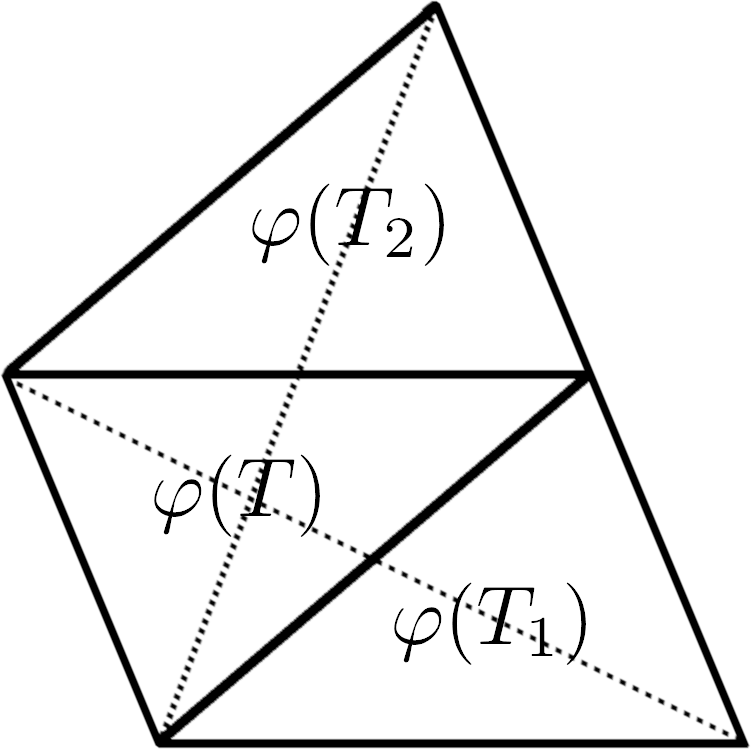
\includegraphics[width=.25\textwidth]{figs/spheretri_plane.png}
			\begin{tikzpicture}[scale=.6,line cap=round,line join=round,>=triangle 45,x=1cm,y=1cm]
\clip(-0.5194903865123804,-2.5120492887047456) rectangle (6.611417807606881,3.221586353864317);
\fill[opacity=0,line width=2pt] (2.7418465885478605,2.9045288146832235) -- (0.4115999626018961,0.44880737041701263) -- (1.56,-2.08) -- (5.58,-2.08) -- cycle;
\draw [line width=2pt] (2.7418465885478605,2.9045288146832235)-- (0.4115999626018961,0.44880737041701263);
\draw [line width=2pt] (0.4115999626018961,0.44880737041701263)-- (1.56,-2.08);
\draw [line width=2pt] (1.56,-2.08)-- (5.58,-2.08);
\draw [line width=2pt] (5.58,-2.08)-- (2.7418465885478605,2.9045288146832235);
\draw [line width=2pt] (4.163979603645924,0.4068967404389632)-- (0.4115999626018961,0.44880737041701263);
\draw [line width=2pt] (4.163979603645924,0.4068967404389632)-- (1.56,-2.08);
\draw [line width=1pt,dotted,opacity=.6] (2.7418465885478605,2.9045288146832235)-- (1.56,-2.08);
\draw [line width=1pt,dotted,opacity=.5] (5.58,-2.08)-- (0.4115999626018961,0.44880737041701263);
-\draw (2.978509173575852,-.8725949117012167) node[anchor=north west] {\large$\varphi(T_1)$};
-\draw (5.078509173575852,-.8725949117012167) node[anchor=north west] {\large$m_1$};
\draw (1.706327414776063,1.5774047550323834) node[anchor=north west] {\large$\varphi(T_2)$};
\draw (3.706327414776063,1.5774047550323834) node[anchor=north west] {\large$m_2$};
\draw (1.2021456159842953,-0.08849580106548587) node[anchor=north west] {\large$\varphi(T)$};
\draw (0.1021456159842953,-0.38849580106548587) node[anchor=north west] {\large$\ell$};
\end{tikzpicture}
			\caption{The image under $\vphi$ of $T,T_1,T_2$ which form the quadrilateral $Q$.}
			\label{fig:sphtris_pl}
		\end{figure}
		

Since $T\cup T_1$ and $T\cup T_2$ are both spherical quadrilaterals which overlap on the spherical triangle $T$, the images of $T\cup T_1$ and $T\cup T_2$ are Euclidean parallelograms of equal area which overlap on a shared triangle $\vphi(T)$.
	Therefore, the image of $T\cup T_1\cup T_2$ must 
	consist of two parallelograms, one of whose 
	edges is the diagonal of the other. In other words, 
	$\vphi(T\cup T_1\cup T_2)$ is a Euclidean trapezoid 
	whose boundary consists of four Euclidean geodesic 
	segments, as in \Cref{fig:sphtris_pl}.
	
	To find the contradiction, consider the point on the sphere shared by $T$, $T_1$, and $T_2$.  Since these triangles are all equilateral spherical triangles, the three angles at this point are each strictly greater than $\tfrac{\pi}{3}$ radians, because the sum of interior angles on a triangle is strictly greater than $\pi$.  
	so, the total measure of the three angles at this point is greater than $\pi$,  Therefore, the two geodesic segments which are part of the boundaries of $T_1$ and $T_2$ meet at this point at an angle of measure strictly greater than 
	$\pi$. Therefore, together they do not form a single geodesic.  On the sphere, the region $T\cup T_1\cup T_2$ has a boundary consisting of five geodesic segments whereas its image has a boundary consisting of four, which contradicts the assumption that $\vphi$ and $\vphi^{-1}$ preserve geodesics.
\end{proof}

This implies that no map projection can preserve the ordering of regions by their convex hull scores, which is what we aimed to show.
\zs{add more discusssion}

\section{Reock}\label{sec:reock}

Let $\mathrm{circ}(\Omega)$ denote the \textit{smallest bounding
circle} (smallest bounding \textit{cap} on the sphere) of a region
$\Omega$.  Then the \textit{Reock score} of $\Omega$ is 

$$\mathrm{Reock}(\Omega)=
\frac{\mathrm{area}(\Omega)}{\mathrm{area}(\mathrm{circ}(\Omega))}.$$

In words, it is the ratio of the area of the region to the area of the
smallest circle containing that region, and it is equal to one if and
only if $\Omega$ is a circle.  We can observe that
$\mathrm{CH}(\Omega)\geq \mathrm{Reock}(\Omega)$, since the convex
hull of a region is never larger than the smallest bounding circle.
This relation holds with equality if and only if the convex hull of
$\Omega$ is a circle.  


Since $\mathrm{Reock}(\Omega)=1$ if and only if $\Omega$ is a circle,
we can observe that any candidate for a map projection which preserves
the ordering of Reock scores must, at the very least, preserve the
maximizeres in the ordering, meaning it sends caps on the sphere to
circles in the plane.  The \textit{stereographic projection} is one
such circle-preserving map projection, and we will show that the
family of map projections which are circle-preserving are exactly
those which can be written as the composition of the stereographic
projection and a \textit{scaled isometry} of the plane.  \mute{

\begin{definition}
The \textbf{stereograpic projection} from the sphere to the plane is
defined by placing the plane tangent to the sphere at the south pole,
and for any point $p$ on the sphere other than the north pole, $p$ is
sent to the unique point $q$ in the plane which is on the line in
3-space passing through the north pole and $p$.

If $(x,y,z)$ is a point on the sphere, then the action of the
stereographic projection is

$$(x,y,z)\mapsto \left(\frac{x}{1-z},\frac{y}{1-z}\right),$$

and its inverse, for $(u,v)$ in the plane:

$$(u,v)\mapsto \left( \frac{2u}{1+u^2+v^2},\frac{2v}{1+u^2+v^2},
\frac{u^2+v^2-1}{1+u^2+v^2}   \right).$$

\end{definition}

What is somewhat surprising is that this projection sends every cap on
the sphere which doesn't pass through the north pole to a circle in
the plane.  There are several proofs of this fact, and we present
a rather straightforward algebraic one here.

\begin{lemma}
The stereographic projection sends every cap which does not pass through the north pole to a circle in the plane.
\end{lemma}
\begin{proof}

We proceed algebraically.  Since a cap on the sphere can be identified
by the plane in $\R^3$ which intersects the sphere along its boundary,
we can parametrize such a cap by writing the equation for its
corresponding plane, $ax+by+cz=d$, restricting $(x,y,z)$ to be points
on the sphere.  The image in the plane of this cap is some set of
$(u,v)$ points, and we can explicitly write this by substituting in
for $x$, $y$, and $z$ the corresponding values for the inverse
stereographic projection.  We write $\mathcal{W}=u^2+v^2$ for the ease
of presentation. 

\begin{align*}
    d&=ax+by+cz\\
    d&=a\left(\frac{2u}{1+u^2+v^2}\right)+b\left(\frac{2v}{1+u^2+v^2}\right)+c\left(\frac{u^2+v^2-1}{1+u^2+v^2}\right), \text{ by substitution}\\
    d&=a\left(\frac{2u}{1+\mathcal{W}}\right)+b\left(\frac{2v}{1+\mathcal{W}}\right)+c\left(\frac{\mathcal{W}-1}{1+\mathcal{W}}\right), \text{ by change-of-variable }\mathcal{W}=u^2+v^2\\
    d\left(1+\mathcal{W}\right)&=2au+2bv+c\left(\mathcal{W}-1\right), \text{ multiplying through by }1+\mathcal{W}\\
    0 &= (c-d)\mathcal{W} + 2au +2bv - c - d,\text{ by rearrangement}\\
    0 &= (c-d)(u^2+v^2)+2au+2bv - c - d,\text{ by change-of-variable } \mathcal{W}=u^2+v^2
\end{align*}

This last line is the equation of a circle in the plane if $c\neq d$ and a line otherwise.  Since $c=d$ if and only if the point $(x,y,z)=(0,0,1)$ (i.e. the north pole) is on the plane, and we assumed that this is not the case, we have shown that the image under the stereographic projection of every cap which does not pass through the north pole is a circle in the plane.

\end{proof}


We now have in-hand a circle-preserving map projection, and we now turn to demonstrating that the stereographic projection is essentially the unique map projection with this property.  We can observe that if we perform stereographic projection and compose it with a transformation of the plane which sends every circle to a circle, then this composition is a circle-preserving map projection.  The next lemma demonstrates that the class of transformations of the plane which preserve circles is actually quite narrow.

\begin{lemma}
If $T$ is a transformation of the plane which sends every circle in the plane to another circle, then $T$ must be a linear transformation which is the composition of a scaling, a rotation, a reflection, and a translation, i.e. a scaled isometry.
\end{lemma}
\begin{proof}

We first argue that if we restrict our attention to \textit{linear} transformations, the scaled isometries are the only transformations which preserve circles.  

If $T$ is a scaled isometry with scaling factor $\alpha$, then, by definition, for any points $x$ and $y$, the distance between $T(x)$ and $T(y)$ is $\alpha$ times the distance between $x$ and $y$.  Therefore, if we choose a circle $Y$ of radius $r$ and let $x$ be the center, then for any $y\in Y$, $d(T(x),T(y)) = \alpha r$, so $T(Y)$ is a circle of radius $r$.

Next, if $T$ is a linear transformation which is \textit{not} a scaled isometry, then we can find three points $x$, $y$, and $z$ such that $d(T(x),T(y)) = \alpha d(x,y)$ but $d(T(x),T(z)) \neq \alpha d(x,z)$.  Furthermore, since linear transformations preserve ratios of lengths of collinear segments, and we have two segments whose ratios of lengths are not preserved, these three points cannot be collinear, so we can consider the circle centered at $x$ and passing through $y$ and $z$.  But, since the ratio of lengths isn't preserved, $T$ distorts this circle, so $T$ is not circle-preserving.

We next need to rule out the existence of a non-linear transformation $T$ which is circle preserving.  We proceed by contradiction.  Suppose that $T$ is non-linear and circle-preserving.  Then, since $T$ is non-linear, there is some line $\ell$ such that the image $T(\ell)$ is not a line, so we can find three points $x$, $y$, and $z$ which are collinear, but $T(x)$, $T(y)$, and $T(z)$ are not.  Therefore, we can find a unique circle $C_T$ passing through $T(x)$, $T(y)$, and $T(z)$.  Let $T(a)$ be some other point on this circle, and we consider the preimage of this point, $a$.  If $a$ is not on the line $\ell$, then we can construct two circles, one passing through $a$, $x$, and $y$ and one passing through $a$, $y$, and $z$.  These two circles intersect at only two points, $a$ and $y$, but both of these circles are sent to $C_T$ by $T$, which is impossible if $T$ is injective.  Therefore, $a$ must lie on the line $\ell$.

By repeating this argument, any point on the circle $C_T$ must be the image of some point on $\ell$.  By continuity, we can see that every point on $\ell$ is sent to a point on $C_T$, but the homeomorphic image of a line cannot be a circle, so such a non-linear $T$ cannot exist.

Thus, a transformation of the plane is circle-preserving if and only if it is a scaled isometry.


\end{proof}

We can put these two pieces together to prove the main tool of this section -- that any map projection from the sphere to the plane which preserves circles is the composition of the stereographic projection and a scaled isometry.

\begin{lemma}
The map projections from the sphere to the plane which send every cap to a circle are exactly those which can be written as the composition of the stereographic projection followed by a scaled isometry of the plane.
\end{lemma}
\begin{proof}
Let $\varphi$ and $\psi$ be two map projections which preserve circles, 
and without loss of generality let $\varphi$ be the standard stereographic projection.  
Then the composition $T=\psi\circ\varphi^{-1}$ is a transformation of the plane which preserves circles, so by the previous lemma, $T$ is a scaled isometry.  Then, we can write 
$\psi= T^{-1}\varphi$, which is the composition of the stereographic projection and a scaled isometry.
\end{proof}

As in the previous section, we can construct an example of two regions whose Reock scores are permuted by the stereographic projection.  In fact, we can use \textit{exactly} the same pair of regions as in the convex hull settings, as is made clear by the following lemma.



\begin{lemma}
Let $\varphi$ be the stereographic projection and $C_\theta$ be a spherical cap centered at the south pole parametrized by the angle $\theta <\pi/4$ formed between the central axis of the sphere and the line of projection passing through the north pole and the boundary of the cap (Figure~\ref{fig:stereocap}). Then $\phi(C_\theta)$ is a disk in the plane, centered at the origin, and has radius $2\tan\theta$
\end{lemma}
\begin{figure}
    \centering
    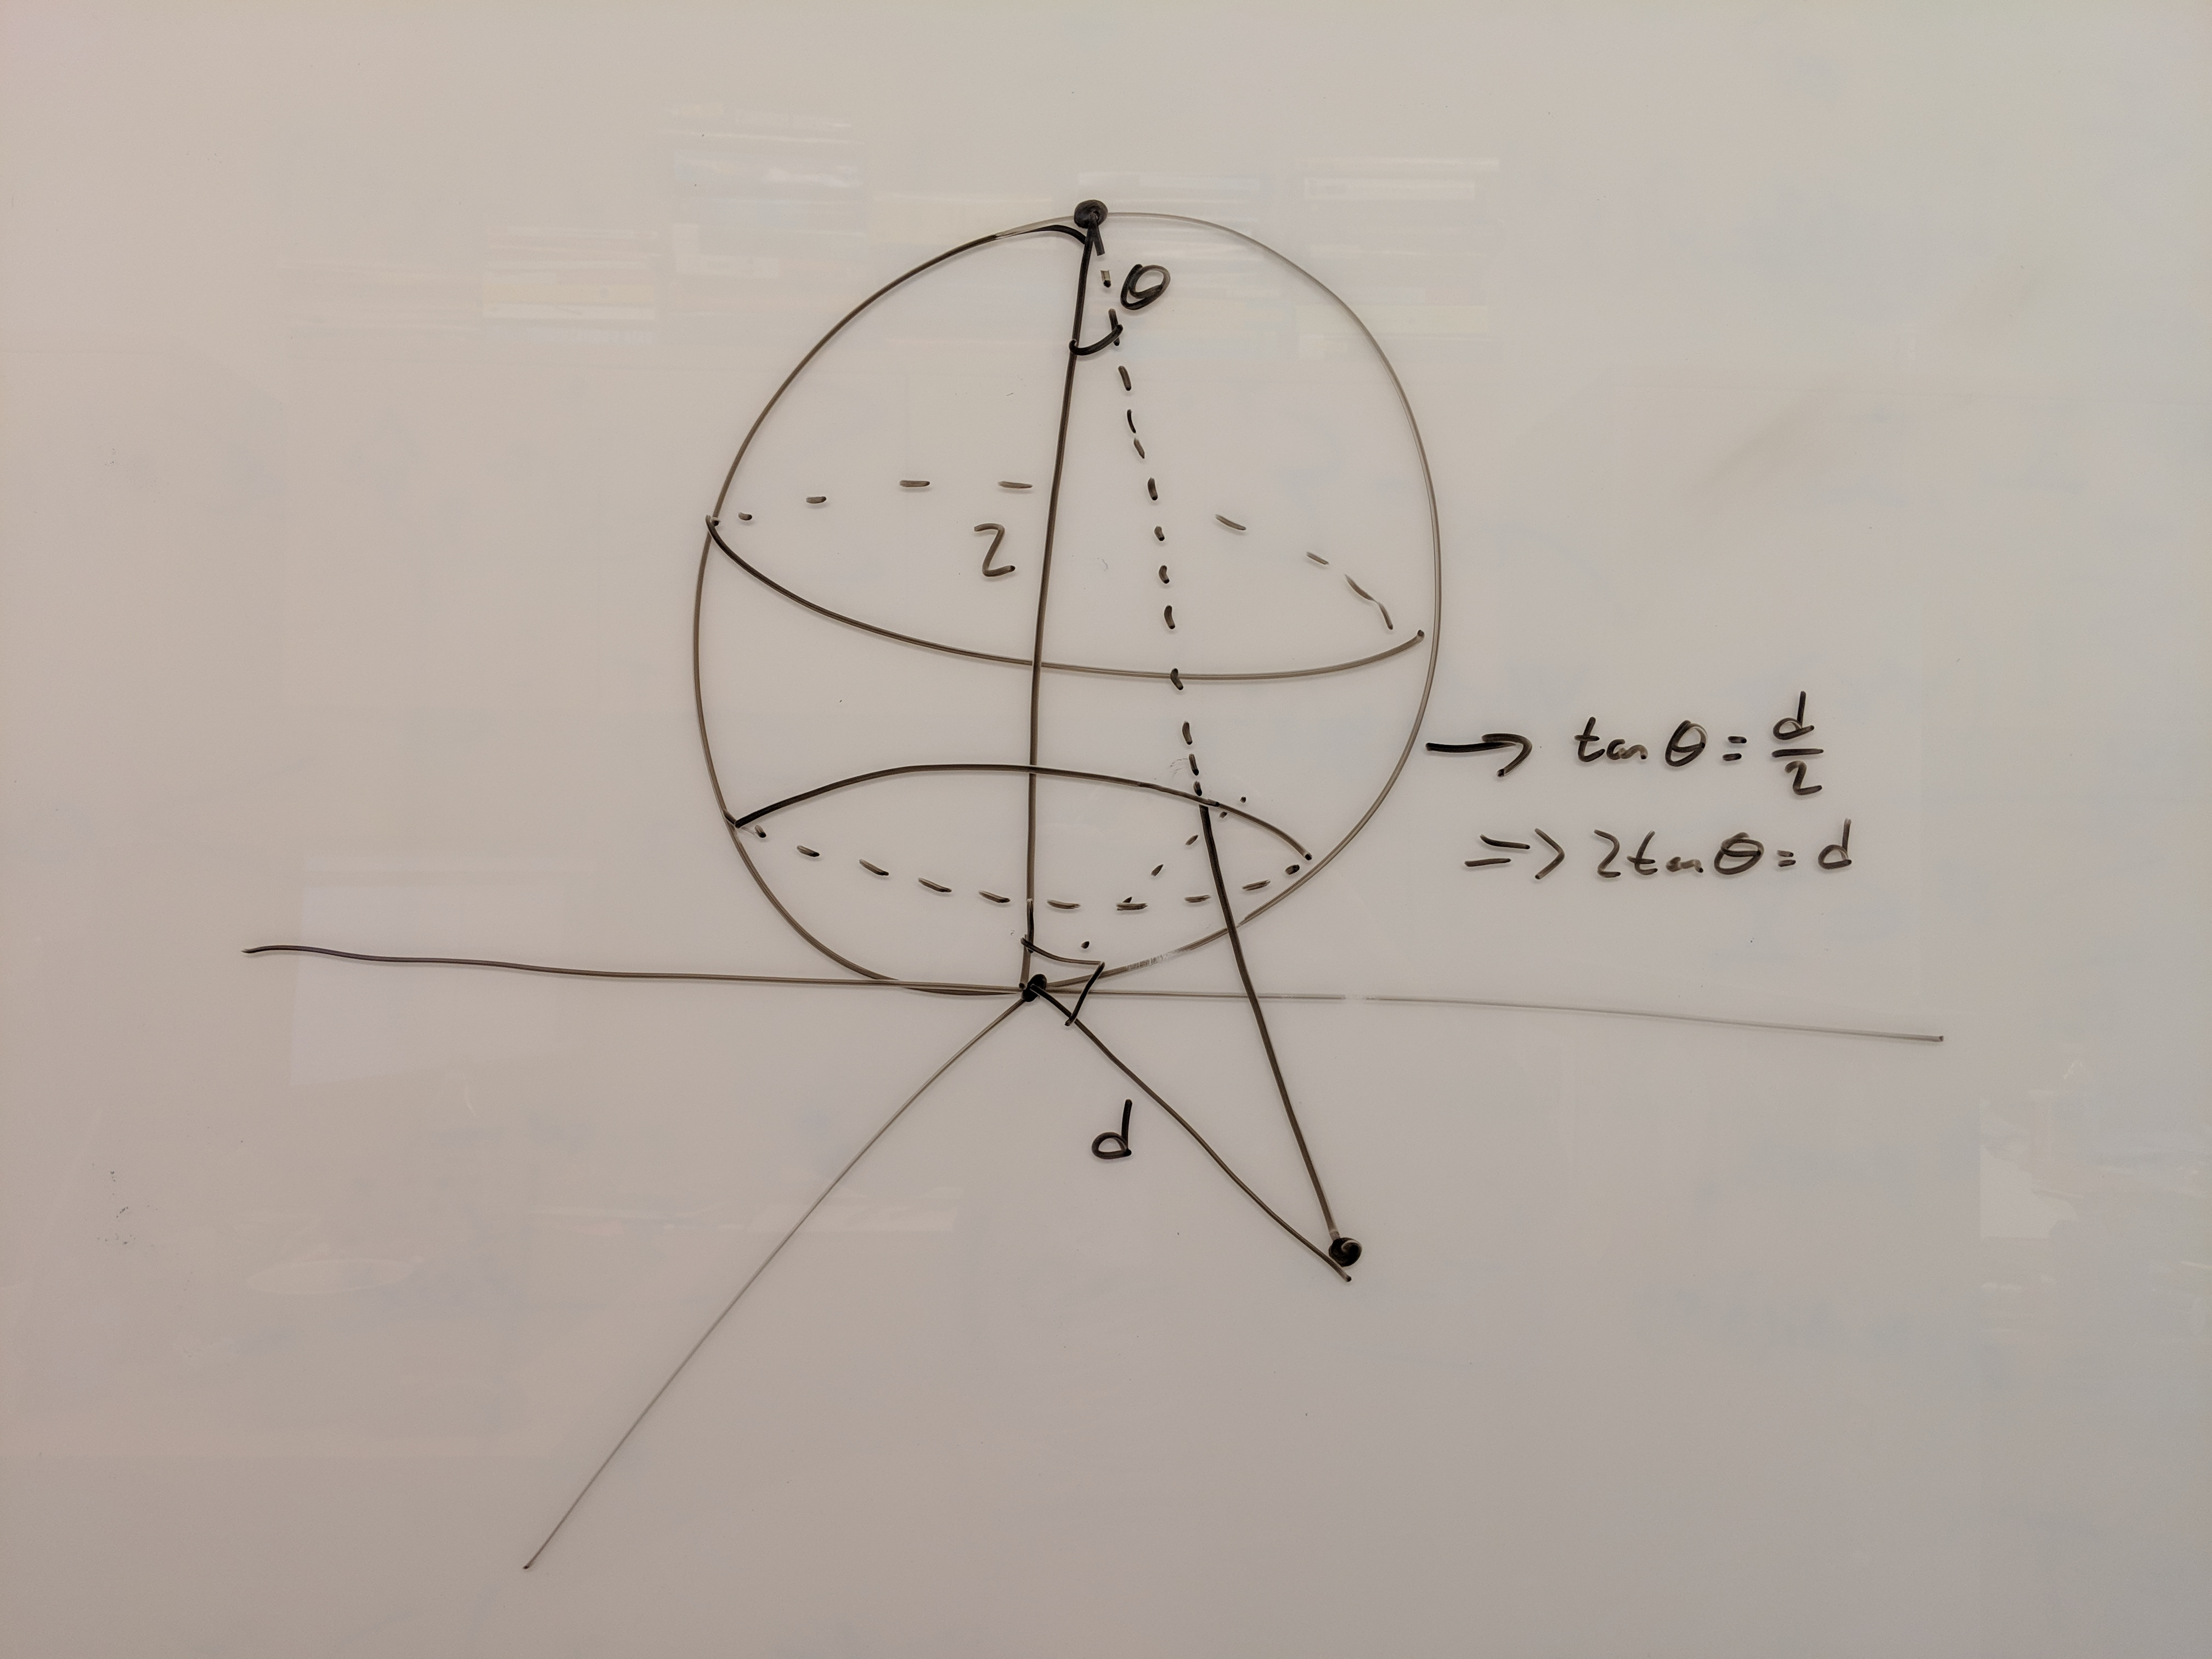
\includegraphics[width=.8\textwidth]{figs/stereo_cap.jpg}\\
    \caption{ The image of a cap with angle $\theta$ between the polar axis and the line of projection is a circle of radius $2\tan\theta$.  }
    \label{fig:stereocap}
\end{figure}
\begin{proof}


Since $\varphi$ projects from the north pole of the sphere and the sphere's south pole is mapped to the origin in the plane, the image of $C_\theta$ is totally radially symmetric about the origin, and is therefore a circle.  To see that its radius is $2\tan(\theta)$, place the south pole of the sphere tangent to the plane at the origin. By construction, for any point $p$ on the boundary of $C_\theta$, there is a unique line passing through the north pole of the sphere, $p$, and the point $\varphi(p)$ on the boundary of the disk in the plane.  By definition, this line meets the central axis of the sphere at an angle of $\theta$, and the central axis of the sphere meets the plane orthogonally, so the center of the sphere, the origin, and the point $\varphi(p)$ form a right triangle with angle $\theta$.  Since we know that the distance between the north pole of the sphere and the origin is 2, we can write the distance between the origin and $\varphi(p)$ as $2\tan(\theta)$.

\end{proof}
}
Since the properties of the stereographic projection near the origin is structurally so similar to that of the gnomonic projection, the exact same pair of regions serves as the counterexample in this setting as well.  When we examine the Reock scores of the projected regions in the plane, the factors of two cancel out.



We now have a concrete example of the stereographic projection permuting scores, by Lemma~\ref{lem:noafflin} in the previous section, since scaled isometries are a special kind of affine linear transformations, they too preserve ratios of areas and therefore Reock scores.  We can conclude this section by summarizing the proof of the main result.

\begin{theorem}
There is no map projetion from the sphere to the plane which preserves the ordering of Reock scores.
\end{theorem}
\begin{proof}
Since such a projection must send caps on the sphere to circles in the plane, it must be the composition of the stereographic projection with a scaled isometry of the plane.  Since scaled isometries preserve Reock scores and therefore their ordering, a Reock score order-preserving projection from the sphere to the plane cannot exist if the stereographic projection does not preserve the ordering.  By the constructed counterexample, it does not, and therefore there is no such Reock score ordering map projection.
\end{proof}
\begin{theorem}\label{thm:reock}
	Let $A$ be a region on the sphere.  Then there exist two regions $\kappa'_N,\kappa'_S\subset A$ such that the Reock scores of $\kappa'_N$ and $\kappa'_S$ are equal on the sphere, but under the stereographic projection $\varphi$, the Reock score of $\kappa'_S$ is strictly greater than that of $\kappa'_N$. 
\end{theorem}


\begin{proof}
	
	The structure of this proof is identical to that of \Cref{thm:convhull}.
	
	First, since $A$ is a region, we can find some cap $\kappa$ inside of $A$ such that the center of $\kappa$ is not the south pole of the sphere, and the north pole is exterior to $\kappa$.  This cap is bisected by a line of longitude, in particular the great circle which passes through the two poles and the center of $\kappa$.  This line of longitude meets $\kappa$ at exactly two points, and we call $p_N$ the point closer to the north pole and $p_S$ the point closer to the south pole.
	
	Choose some $r$ strictly less the radius of $\kappa$ and let $\kappa'_S$ be the region constructed by deleting a cap of radius $r$ from the interior of $\kappa$ tangent at $p_S$.  Construct $\kappa'_N$ analogously by deleting a cap of radius $r$ tangent at $p_n$. Observe that the Reock scores of $\kappa'_N$ and $\kappa'_S$ are identical, since each has the boundary of $\kappa$ as its smallest bounding cap and both figures have the same area.
	
	We now consider the images of $\kappa'_N$ and $\kappa'_S$ under the stereographic projection $\varphi$.  Since $\varphi$ preserves points of tangency, containment, and sends every cap away from the north pole to a circle, the images $\varphi(\kappa'_N)$ and $\varphi(\kappa'_S)$ are both regions which are disks with a smaller disk, tangent to a point on the circumference, deleted.  Furthermore, since the boundary of $\kappa$ was the smallest bounding cap of both regions on the sphere, the image of the boundary of $\kappa$ under $\varphi$ is the smallest bounding circle of the images of these regions in the plane.
	
	We can now observe that these two regions in the plane do not have the same Reock score.  Both have the same bounding circle, but $\varphi(\kappa'_N)$ is strictly smaller than $\varphi(\kappa'_S)$.  This is because the stereographic projection distorts areas in a way such that figures further from the south pole have their areas magnified more than the same region closer to the south pole.  If the regions in question are sufficiently small, letting $\theta$ denote the polar angle at which we consider a small cap on the sphere, a cap of radius $r$ will be sent to a circle with radius roughly $r/\cos^2{\theta}$\zs{check  this}, and a straightforward examination of this as a function of $\theta$ shows that it grows faster as $\theta$ increases.
	
	Since $\varphi(\kappa'_N)$ fills a smaller fraction of the bounding circle than $\varphi(\kappa'_N)$ does, its Reock score is strictly worse, and the stereographic projection does not preserve Reock scores.
\end{proof}
\section{Isoperimetric Quotient}\label{sec:isoper}

\zs{The proof here is pretty informal.  I don't know if it's worth doing; the calculus needed is super gross. }

\zs{One way we can include this without having to compute a bunch of path integrals is to move the Polsby-Popper section to after Reock, then this can be rolled into that section as part of the `discussion' or whatever.}

We remarked at the end of Section~\ref{sec:pp} that a more principled version of an isoperimetric quotient may avoid the failure of the ordinary Polsby-Popper score to induce an ordering which can be preserved by some map projection.

\begin{definition}
We define the \textbf{isoperimetric quotient score} of a region $\Omega$ to be$$
\mathrm{IPQ}(\Omega)=
\begin{cases}
\frac{4\pi \ \mathrm{area}(\Omega)}{\mathrm{perim}(\Omega)^2} \text{ in the plane},\\[10pt]
\frac{\mathrm{area}(\Omega)^2 - 4\pi \ \mathrm{area}(\Omega)}{\mathrm{perim}(\Omega)^2}\text{ on the sphere}
\end{cases}
$$
\end{definition}

This score properly resolves the issue of scale-noninvariance, and the isoperimetric quotient scores of circles in the plane \textit{and} caps on the sphere are one, regardless of their size.

We'll prove order non-preservation in the same way as before, and we built all of the machinery needed to do it in the previous section.  Since any order-preserving map projection needs to preserve the maximizers and caps and circles maximize the isoperimetric quotient score, we can restrict our attention to map projections which send caps to circles.  We showed in the previous section that these are exactly the projections which are the composition of the stereographic projection and a scaled isometry of the plane.  Since this score is scale-invariant, it is preserved by scaled isometries, so we only need to demonstrate the existence of regions on the sphere whose scores are permuted by the stereographic projection.


\begin{theorem}
There exist two regions on the sphere $A$ and $B$ such that $\mathrm{IPQ}(A)>\mathrm{IPQ}(B)$ but under the stereographic projection $\varphi$, $\mathrm{IPQ}(\varphi(A)))<\mathrm{IPQ}(\varphi(B))$.
\end{theorem}

\begin{figure}
    \centering
    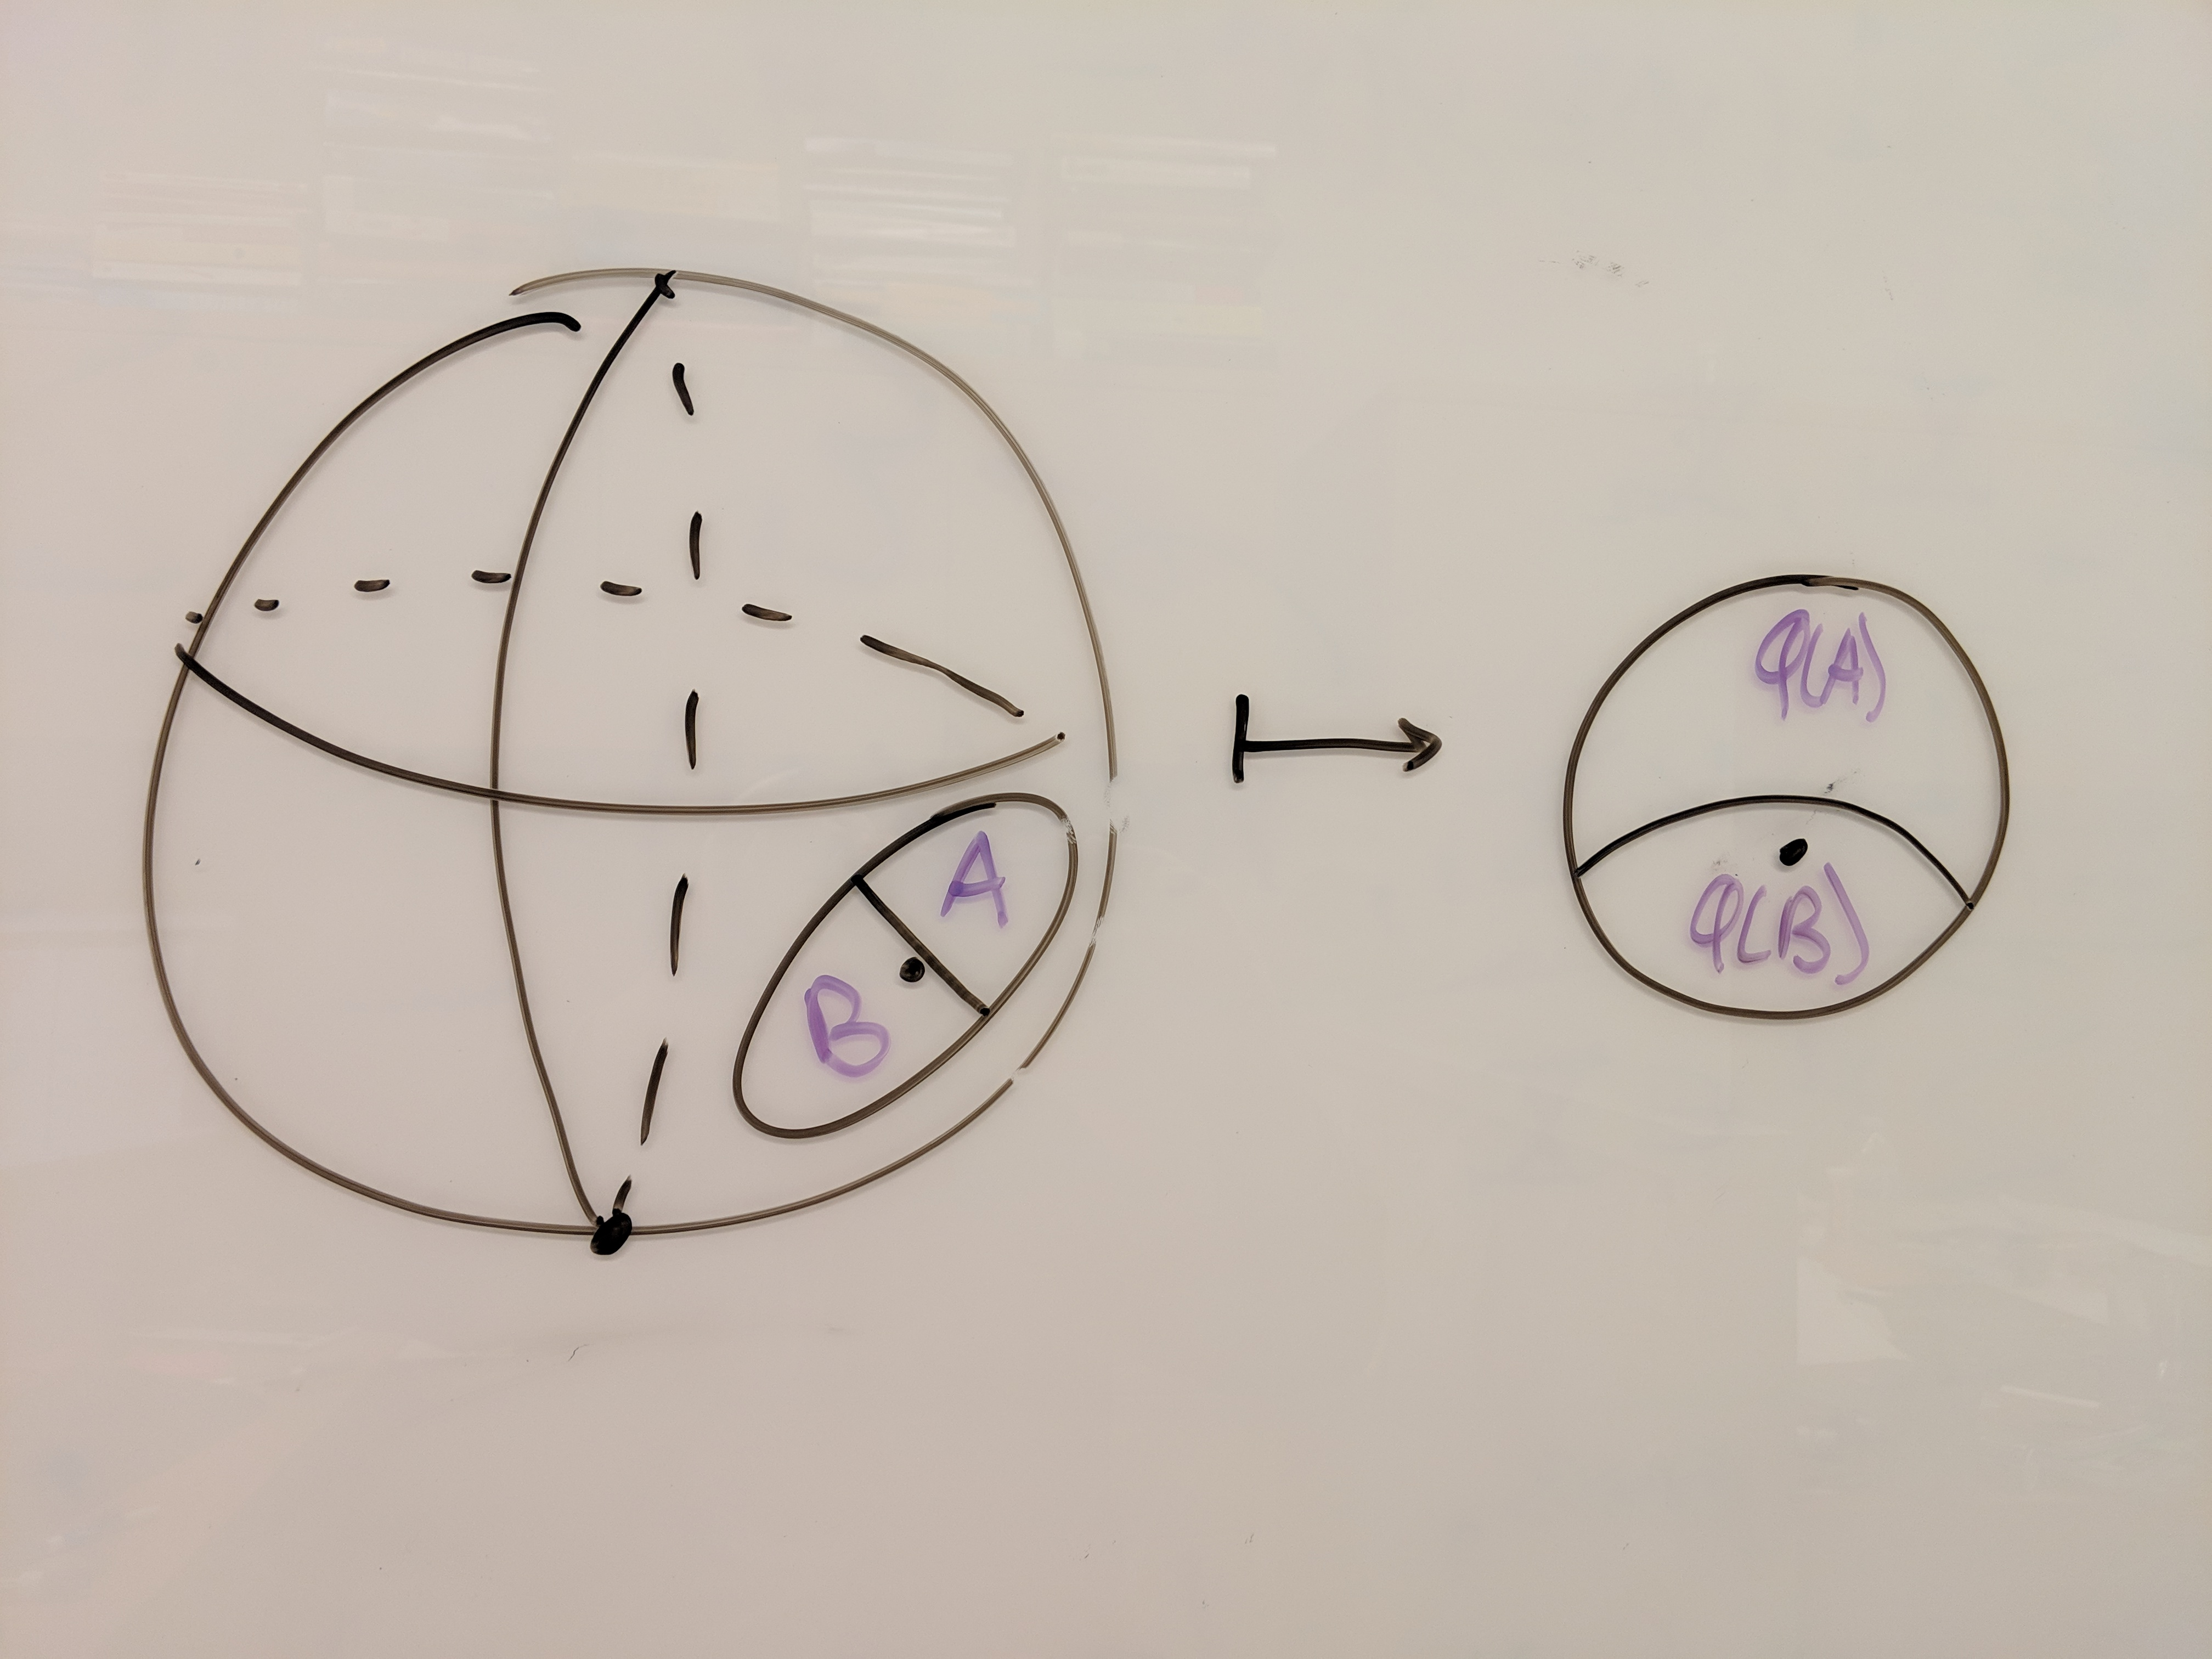
\includegraphics[width=.8\textwidth]{figs/stereo_ipq.jpg}\\
    \caption{ The image of a cap away from the south pole under the stereographic projection. }
    \label{fig:stereoipq}
\end{figure}



\begin{proof}
Let $C$ be a cap with its center slightly away from the south pole, and divide it into a `top' and `bottom' half with the plane that meets the great circle connecting the poles and cap's center orthogonally.  This divides the cap into two pieces with equal area and perimeter, and therefore equal isoperimetric quotient scores.  Shift this division line down so that the top part of the circle has a slightly higher than the bottom.  We let the top part be $A$ and the bottom be $B$.  The stereographic projection sends caps to circles, but does not preserve the \textit{centers} of such caps away from the south pole, and will send the slightly perturbed division line to a nearly circular arc (Figure~\ref{fig:stereoipq}).  

If we had used the original division of the cap into exact halves, then in the plane, the isoperimetric quotient score of $\varphi(A)$ would be strictly less than that of $\varphi(B)$. Since we can choose our perturbation to be small enough to not reverse this order, we have constructed our example of a pair of regions whose isoperimetric score order is not preserved by the stereographic projection.

\end{proof}


The remainder of the argument follows from our previous results.  Lemma~\ref{lem:noafflin} says that no scaled isometry can correct for the permutation of score ordering, so there does not exist a map projection which preserves the ordering over regions induced by the isoperimetric quotient score.







\section{Empirical Results}\label{sec:exper}




The proofs in the previous sections were done with respect to the \textit{unit sphere}.  Although mathematically the results remain equally true for a sphere of radius $\mathcal{R}$, a natural question to raise is whether they remain \textit{practically} true in this setting.  If we view the idealized Earth as a sphere with  $\mathcal{R}=4000\text{ miles}$ and observe that the regions we are often interested in measuring are relatively small compared to the total surface area, then it could be the case that any map projection still distorts the scores of the regions, but not by enough to change their ordering.  Here, we demonstrate that this is not the case, and that in practice the Polsby-Popper, convex hull, and Reock scores of the real Congresional districts are reordered by the map projections used in practice.\footnote{The code to compute the various compactness scores is based on Lee Hachadoorian's \textit{compactr} project \cite{hachadoorian2018reock}.}

Rather than computing the scores on the sphere, we compare the scores a pair of familiar map projections.  Since for any pair of map projections, if the induced score ordering under them is different, then at least one of the two projections must have permuted the score ordering.  The projections we compare are the \textit{Mercator} projection and the \textit{Latitude-Longitude} projection.  The Mercator projection is a cylindrical projection constructed by placing the sphere in the middle of a cylinder and projecting each point on the sphere outward onto the surface of the cylinder along the line passing through the point and the center of the sphere (see Figure~\ref{fig:mercator}).

\begin{figure}
    \centering
    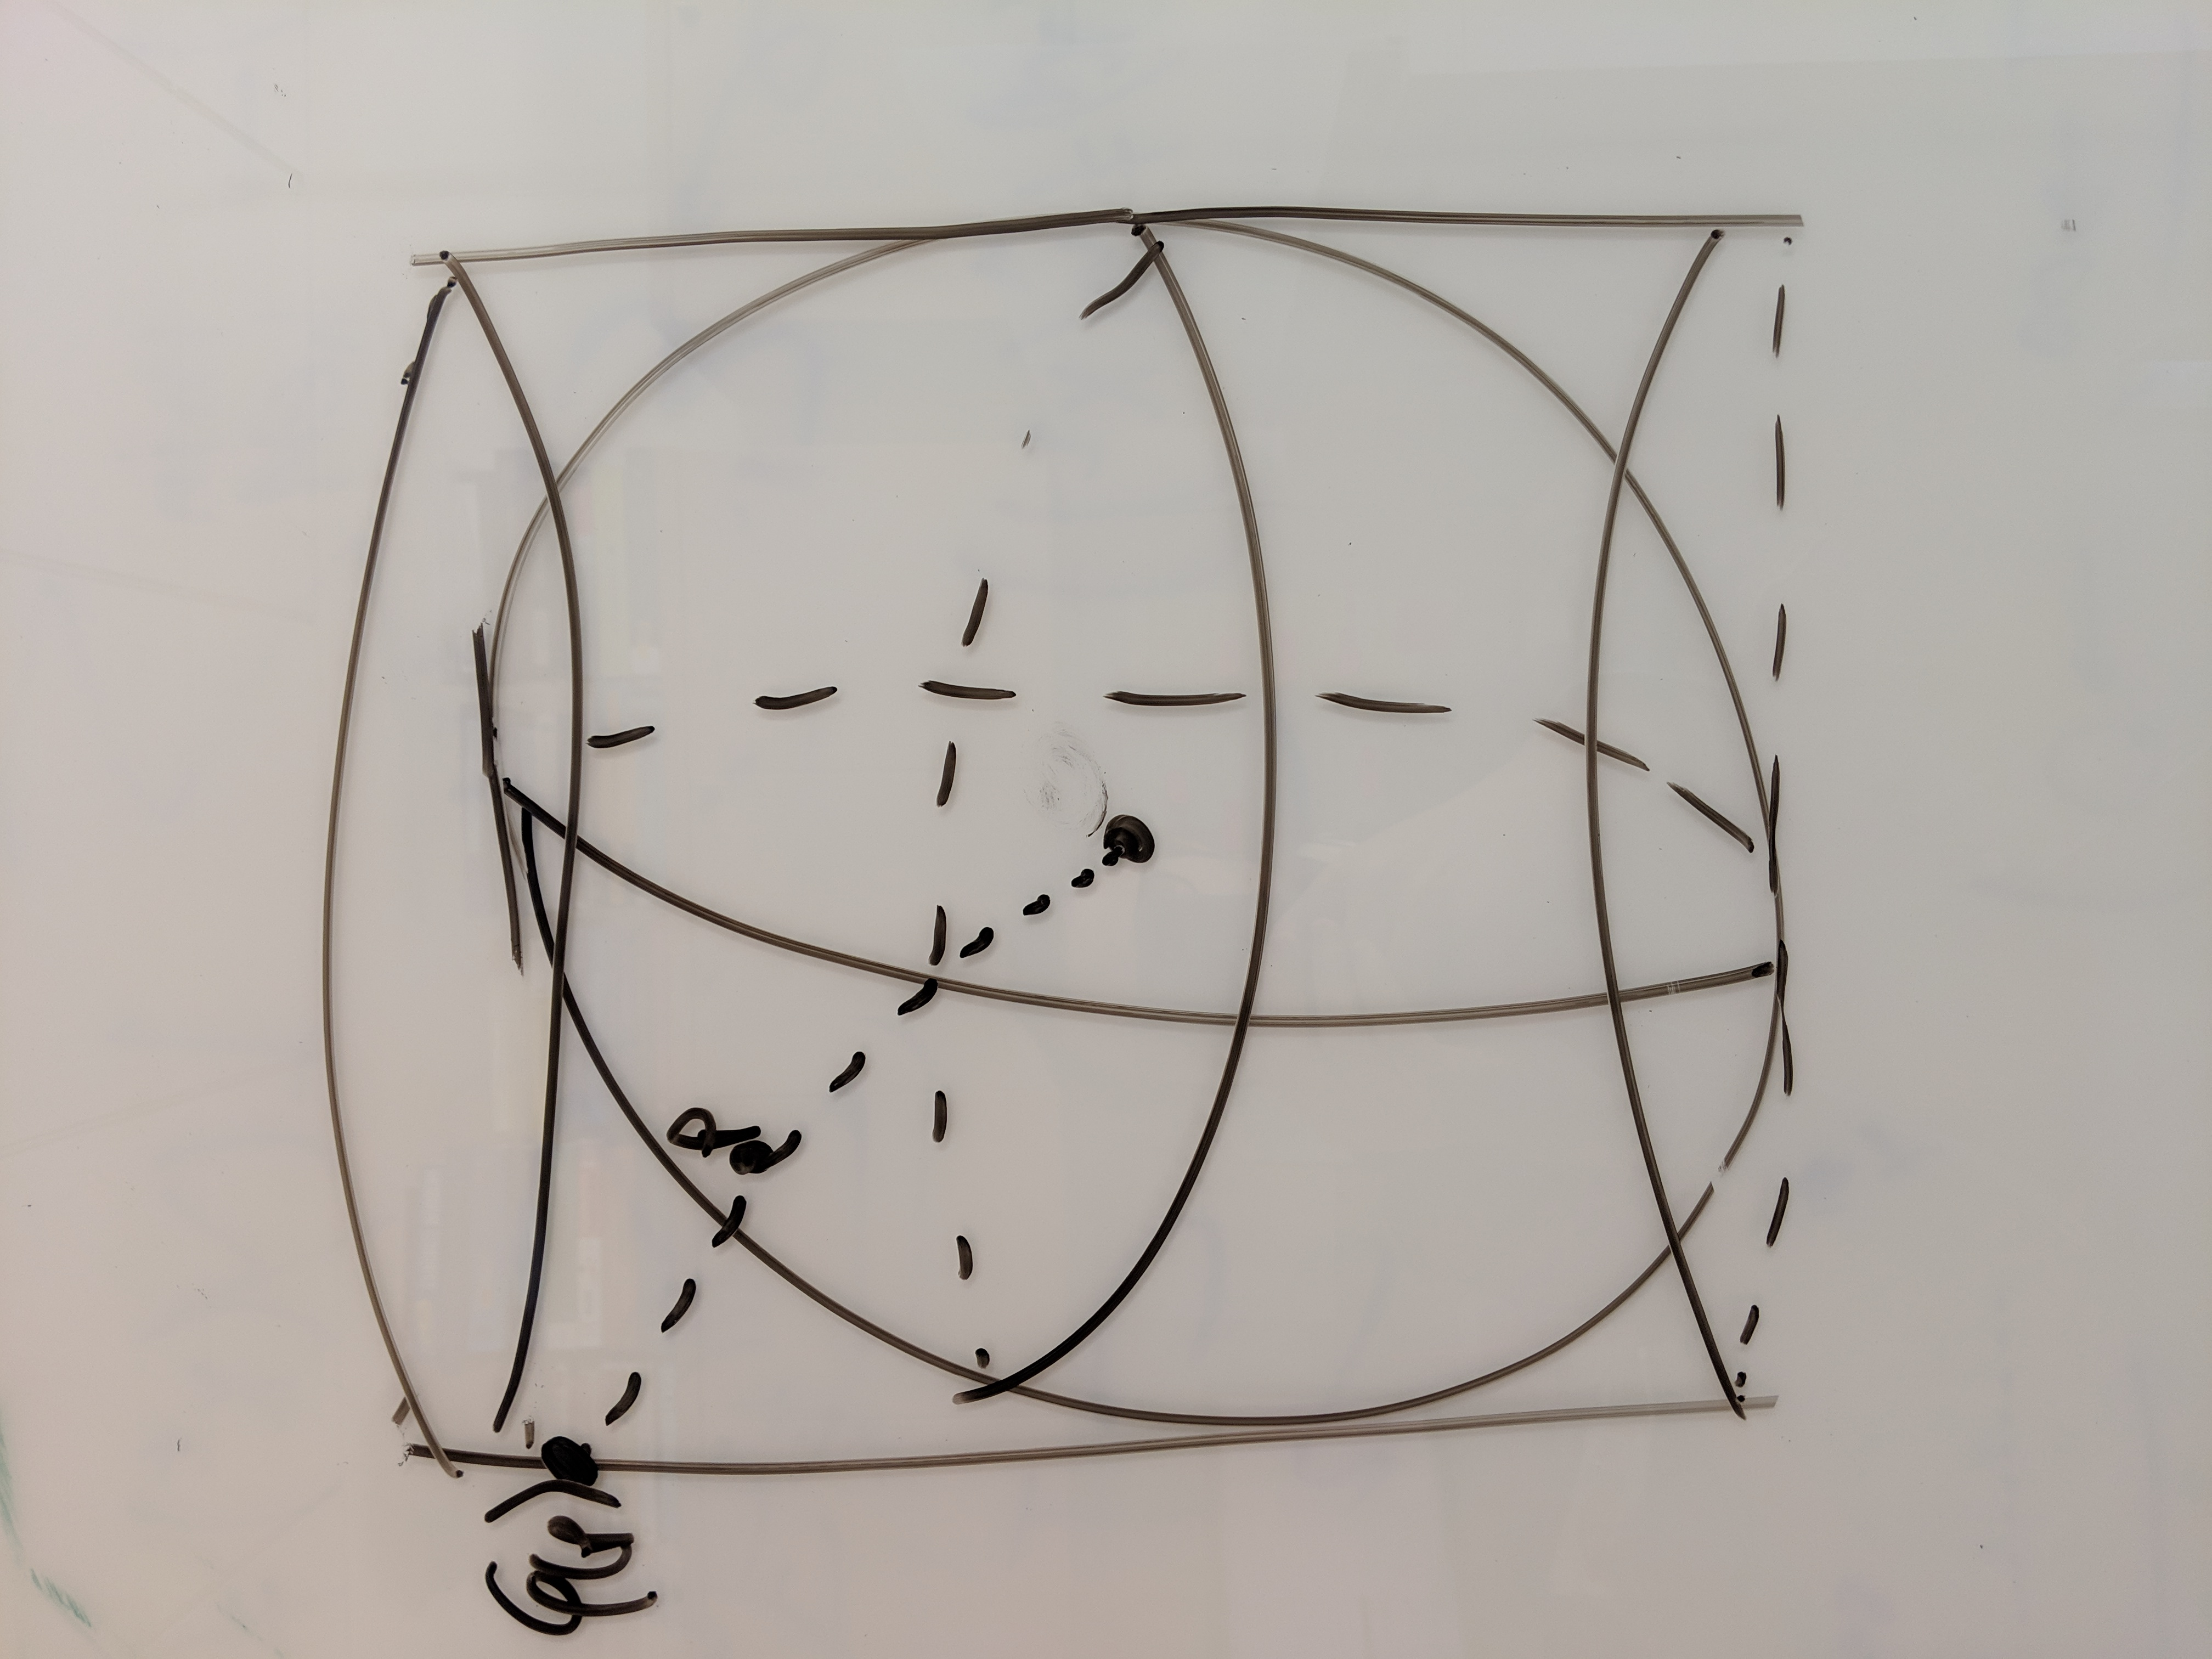
\includegraphics[width=.8\textwidth, angle=270,origin=c]{figs/merc.jpg}\\[1.5em]
    \caption{ A Mercator projection from the sphere to the surface of the cylinder.}
    \label{fig:mercator}
\end{figure}

This cylinder is then `unrolled' to a flat, planar map.  The Latitude-Longitude projection simply uses $(\mathit{\mathrm{lon}},\mathit{\mathrm{lat}})$ pairs as $(x,y)$ coordinates in the plane.  The Mercator and its variants, including the Universal Transverse Mercator and several state plane projections, is among the most commonly used projections.  The U.S. Census Bureau provides shapefiles for geographic entities in the United States, including Congressional districts, in a Latitude-Longitude coordinate reference system.\footnote{We use the U.S. Census Bureau's shapefile for the Congressional districts for the 115th Congress.  These are the districts in place for the 2016 election cycle.  Our Mercator projection is the WGS84 Spherical Mercator (EPSG:3857).  Our Latitude-Longitude projection is the NAD83 North American Latitude-Longitude (EPSG:4269).}


We first compare the three scores under the two projections for all\footnote{An astute reader will notice these plots have 434, points.  We omit the Alaska At-Large Congressional district since it crosses the International Date Line, which makes the convex hull and bounding circle hard to compute in a Latitude-Longitude projection.} districts in the country.  Each point represents one district.  The horizontal axis is the ordinal position with respect to the ordering induced by the score under the Latitude-Longitude projection and the vertical axis under the Mercator projection.  If both projections were to induce the same score ordering, every point would lie on the 45 degree line up the diagonal.


\begin{figure}[H]
\centering
\subfloat[Polsby-Popper]{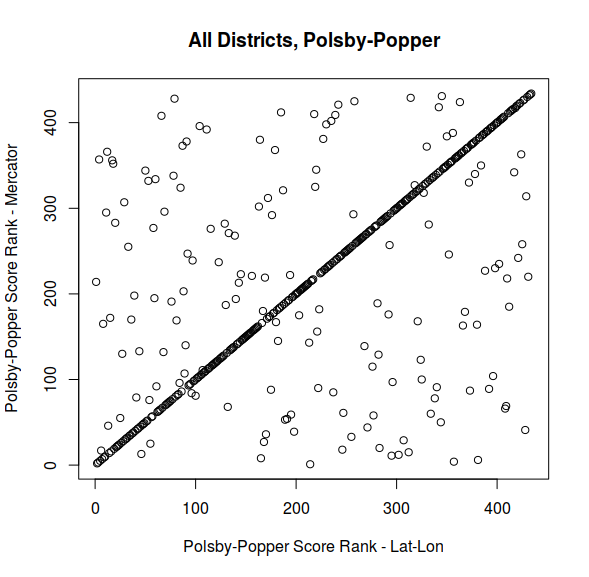
\includegraphics[width = .3\textwidth]{figs/all_pp.png}} 
\subfloat[Convex Hull]{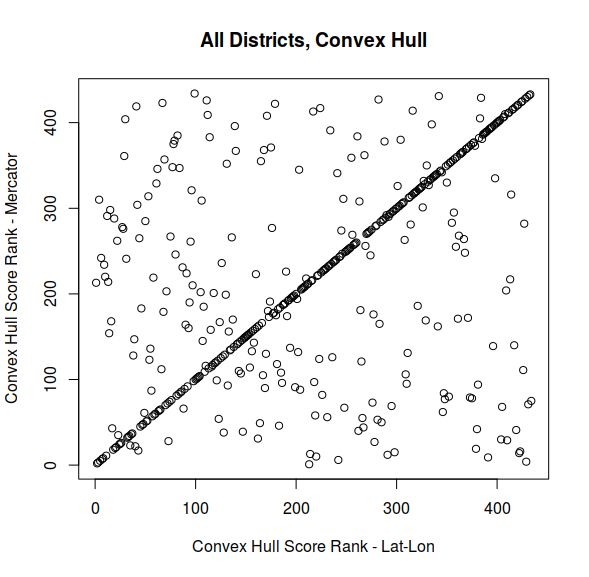
\includegraphics[width = .3\textwidth]{figs/all_ch.png}}
\subfloat[Reock]{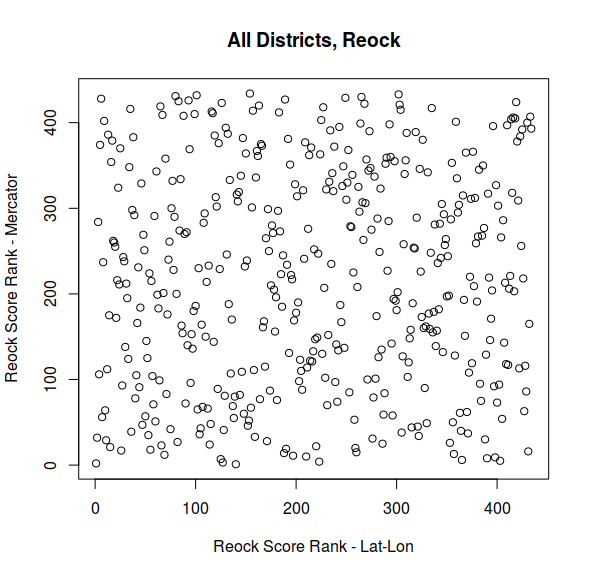
\includegraphics[width = .3\textwidth]{figs/all_reock.png}}\\[1.5em]

\caption{The permutation of compactness scores for all Congressional districts.}
\label{fig:allscores}
\end{figure}



While it is an illuminating exercise to demonstrate this effect across all districts, districting plans are proposed and evaluated on a state-by-state basis.  In the following plots, we restrict our attention to Texas, and observe a similar phenomenon.


\begin{figure}[H]
\centering
\subfloat[Polsby-Popper]{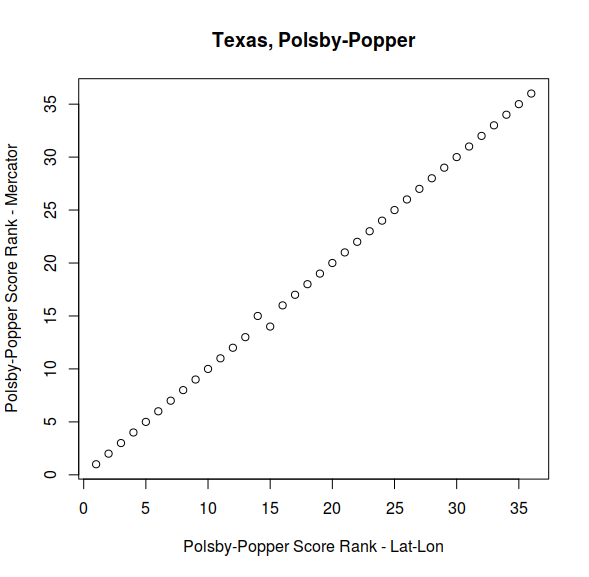
\includegraphics[width = .3\textwidth]{figs/texas_pp.png}} 
\subfloat[Convex Hull]{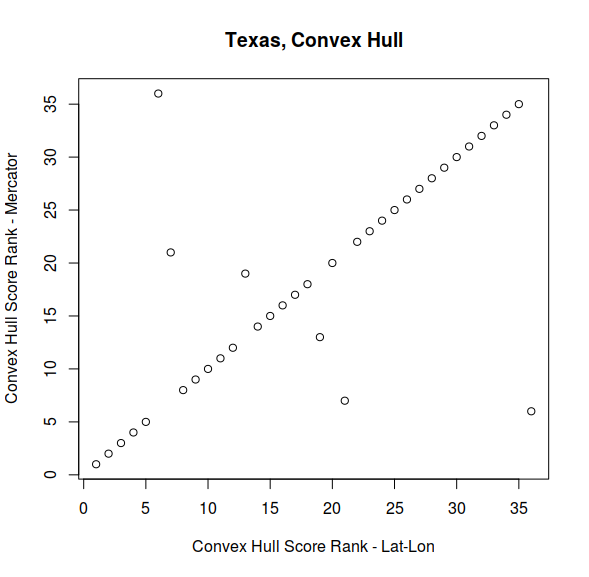
\includegraphics[width = .3\textwidth]{figs/texas_ch.png}}
\subfloat[Reock]{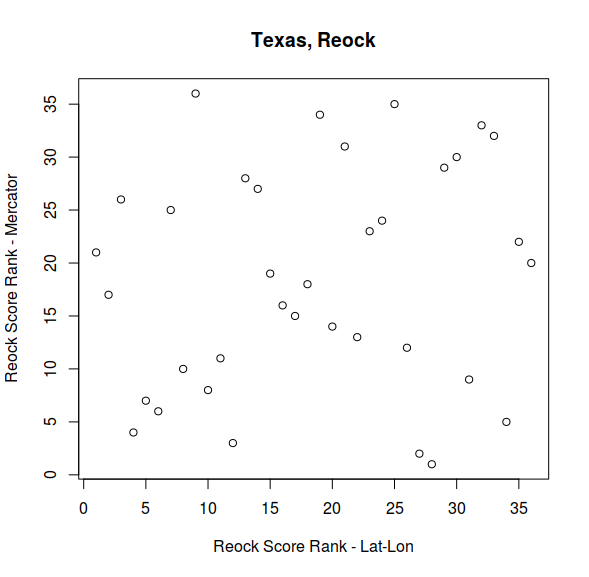
\includegraphics[width = .3\textwidth]{figs/texas_reock.png}}\\[1.5em]

\caption{The permutation of compactness scores for Texas' Congressional districts.}
\label{fig:txscores}
\end{figure}




We observe overall that the orderings of under the Polsby-Popper score and convex hull score are relatively undisturbed compared to that of the Reock score.  This is because the \textit{values} of those scores do not change by too much under different projections.  Intuitively, this is because while both projections distort shapes, they do so in a way that does not affect either of these scores by too much, since in the case of the Polsby-Popper score, the perimeter and area of the regions are changed in similar ways, and in the case of the convex hull score, the area of the convex hull of a region is distorted in the same way as the region itself, so the ratio of the areas is similar across projections.

However, the Reock score specifically requires constructing a minimum bounding circle, and this circle can be dramatically different under different map projections.  The Mercator projection sends caps on the sphere which aren't too close to the poles to regions in the plane which are very nearly circular, while the Latitude-Longitude projection visibly stretches all but the smallest circles on the equator.  For regions away from the equator, such as U.S. Congressional districts, this difference is significant enough to permute the ordering of Reock scores.


\zs{would be cool if we could make a Jupyter notebook or something available with this}
\section{Conclusion and Future Directions}\label{sec:future}
We demonstrate here the failure of a standard panel of compactness measures to provide a consistent score ordering over all regions.  
While compactness scores are not used critically in a \textit{legal} context, they appear frequently in the popular discourse about redistricting issues and frame the perception of the `fairness' of a plan.  For example, a 2014 Washington Post piece  \cite{ingraham2014solve} describes an algorithm which generates highly compact districts because it ignores all of the social and demographic data which are crucial to the process.  The equating of `solving' gerrymandering with generating highly compact districts presupposes that the mathematics used to evaluate the geometric features of districts are unbiased and unmanipulable, and we demonstrate here that this is certainly not the case.


The results here suggest that more nuanced models of compactness are worth exploring.  Graph-theoretic (i.e. `discrete') compactness measures as in \cite{deford2018tv,duchin2018discrete} are computed without reference to any particular metric embedding, so they definitionally cannot be affected by the choice of map projection.  Multiscale measures of compactness as in \cite{deford2018tv} provide a higher resolution view of the geometry of regions.  The authors there leave open the question of to what degree a region's total variation profile is unique, and a strongly positive result to that problem would suggest that you can't ``hide'' any of the geometry of a region using the choice of map projection.

This work opens several promising avenues for further investigation.  We prove strong results for the most common compactness scores, but the question remains what the most general mathematical result in this domain might be, such as giving a set of necessary and sufficient conditions for a compactness score to not induce a permuted order for some choice of map projection.  Generalizing these results to other surfaces and non-standard measures (such as weighting by population) may also be an avenue for examination.


\bibliographystyle{plainnat}
\bibliography{bib.bib}

\end{document}
